%Autor: miguev
%sergio_garcia_reus: 25
%miguev: 2

\chapter{\LyX}
\label{lyx.tex}
\index{\LyX}

% La mayoría de los procesadores de textos están basados en la filosofía
% WYSIWYG (what you see is what you get, lo que ves es lo que tienes) en
% la que el usuario no sólo  tiene que escribir sino también preocuparse
% de dónde aparacerá  cada elemento en el documento final.  Esto lleva a
% conservar prácticas antiguas provenientes  de las máquinas de escribir
% mecánicas. Entre  estas prácticas  todos conocen los  tabuladores, los
% guiones para partir palabras al final de línea, dejar varias líneas en
% blanco para rellenar, etc. Todo eso es definitivamente prediluviano.

% \LyX, a  diferencia de los demás  procesadores de texto, es  lo que se
% denomina un  programa WYSIWYM (what you  see is what you  mean, lo que
% ves es lo que quieres decir).  Esta filosofía de hacer un documento se
% basa  en que  el usuario  no debe  preocuparse de  la composición  del
% texto, sino únicamente del contenido. Es el programa quien se ocupa de
% encajar todo en el papel para que quede bien.

% \LyX~  utiliza \LaTeX,  de modo  que los  conocimientos de  \LaTeX~ se
% pueden utilizar  también en  \LyX. Sin embargo  no se  necesita ningún
% conocimiento de \LaTeX~ para manejar  \LyX, aunque lo que sí necesitas
% es aprender  los conceptos y la  mentalidad de la forma  de trabajo de
% \LyX~  y \LaTeX:  sólo  debes preocuparte  de  escribir el  contenido,
% \LyX~  se encargará  del trabajo  de  formato y  composición de  forma
% consistente.

\LyX,  proporciona  estupendo tutorial  en  castellano  que son  ayuda
suficiente para comenzar a escribir  apuntes, trabajos, cartas y otros
documentos  sin  necesidad  de  estudiar nada  complicado.  Para  leer
la  introducción  o  el  tutorial  de  \LyX~  basta  con  elegir  {\sf
Tutorial} respectivamente en el menú {\sf  Ayuda}. En el mismo menú se
encuentran los  restantes capítulos  de la  documentación de  \LyX~ en
inglés: {\sf Guía del usuario}, {\sf Características extendidas}, {\sf
Personalización}, {\sf Manual  de referencia} y {\sf  Preguntas de uso
frecuente}.

Lo que sigue es el resultado  de modificar la traducción al castellano
del  tutorial de  \LyX, escrito  por  {\sc Sergio  García Reus},  para
adecuarla  al estilo  de este  libro. Aunque  esto es  suficiente para
defenderte  con  \LyX{} te  recomendamos  que  te leas  la  traducción
original.

% No  hay  mucho  que  explicar  de  \LyX~ que  no  esté  en  su  propia
% documentación, así que para no engrosar este libro más de lo necesario
% ni duplicar esfuerzos,  te remitimos a la  excelente documentación que
% incorpora \LyX.

% \begin{figure}[hbtp]
% \centering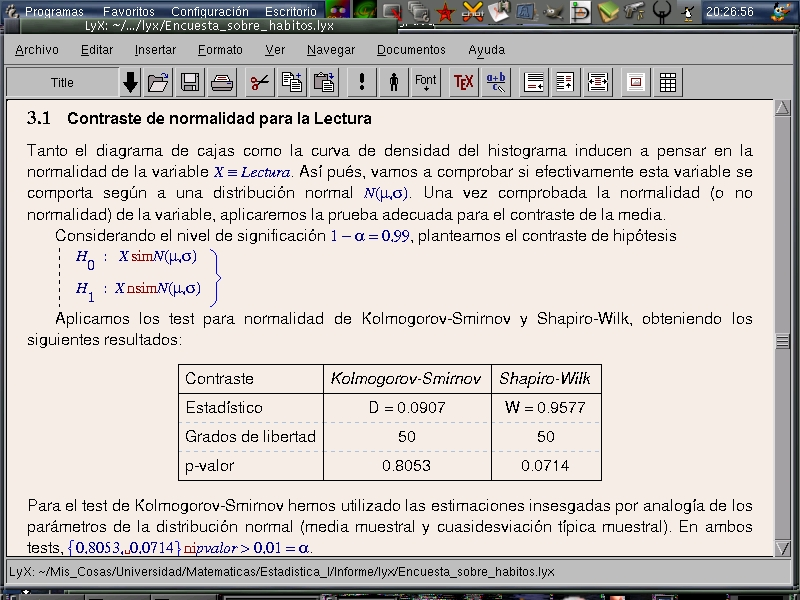
\includegraphics[width=\textwidth]{imagenes/lyx.eps}
% \caption{\LyX~ con un trabajo académico sobre inferencia estadística}
% \end{figure}

\section{¡Bienvenido a \LyX{}!}

Este fichero ha sido diseñado para todos aquellos que nunca han oído
hablar de \LaTeX{}, o no lo conocen muy bien. No tengas miedo, no
tendrás que aprender \LaTeX{} para poder usar \LyX{}. Ese es, al fin
y al cabo, el punto fuerte de \LyX{}: proporcionar un interfaz casi
WYSIWIG (\emph{What You See Is What You Get}) para \LaTeX{}. Sin embargo,
hay algunas cosas que necesitarás aprender para usar \LyX{} de forma
eficiente.

Probablemente has acabado consultando este documento porque has intentado
poner dos espacios después de un punto, o tres líneas en blanco entre
dos párrafos. Tras mucha frustración, has comprobado que no se puede.
De hecho, descubrirás que la mayoría de los pequeños trucos que estabas
acostumbrado a usar con otros procesadores de texto no funcionan en
\LyX{}. La razón es que la mayoría de los procesadores de texto que
has usado hasta ahora necesitaban que el usuario hiciera a mano todo
el espaciado, los cambios de tipo de letra, etc. Así, no sólo se escribía
el documento, sino que además se acababa realizando todo el trabajo
de formato y composición. \LyX{} realiza este trabajo por tí de forma
consistente, dejando que te centres en lo más importante: el contenido
del documento.

Así pues, ten paciencia con nosotros y sigue leyendo. Merece la pena
que leas este tema.


\subsection{Qué \emph{es} este tema y qué \emph{no} \emph{es}}

Antes de  que empecemos  con esta sección,  queremos hacer  un pequeño
apunte. El \emph{Tutorial} usa las convenciones tipográficas señaladas
en la página \pageref{convenciones_tipograficas} Si has llegado a este
manual primero, ve y lee las convenciones tipográficas. Sí, ahora.

Una vez que ya sabes qué significa cada tipo de letra, vamos a hablar
un poco sobre la finalidad de este \emph{Tutorial}.


\subsubsection{Para aprovechar al máximo el tema}

Este \emph{Tutorial} se compone de ejemplos y ejercicios. Para obtener
el máximo provecho de este documento, deberías leerlo todo, tecleando
todos los pequeños detalles que te vayamos explicando (por simples
que sean) e intentando hacer todos los ejercicios para comprobar que
lo entiendes. 

% Por comodidad, puede interesarte imprimir la versión PostScript® de este documento.

Si estás familiarizado con \LaTeX{}, probablemente podrás leer el
\emph{Tutorial} más deprisa, ya que muchas de las ideas de \LyX{}
son realmente ideas de \LaTeX{} disfrazadas. No obstante, \LyX{} no
tiene peculiaridades%
\footnote{o dicho de manera más optimista, {}``características''%
} que tengas que aprender. Incluso aunque no te apetezca leer el resto
del \emph{Tutorial}, harías bien en mirar la sección \ref{sec:latexusers},
que ha sido escrita específicamente para usuarios experimentados de
\LaTeX{}.

La sección \ref{sec:what-is-lyx} ha quedado sin actualizar de una
versión anterior del \emph{Tutorial}, y es un poco general. Aún así,
es una buena introducción {}``panorámica'' a \LyX{}, así que deberías
echarle un vistazo para ir haciéndote una idea sobre él.


\subsubsection{Qué \emph{no} vas a encontrar}

\begin{itemize}

% \item Las lecciones masticadas y dadas de comer con cuchara.

% La tendencia actual%
% \footnote{Nota de \noun{John} Weiss: \ldots{}bueno, al menos en Estados Unidos,
% donde reducimos todo al mínimo común denominador\ldots{}%
% } en la literatura autodidacta informática parece ser: {}``Se asume
% que el usuario tiene el coeficiente intelectual de un mosquito''.
% Nosotros no vamos a hacer eso. 

% Por otro lado, somos conscientes de que la mayoría de los usuarios
% acuden a un manual, especialmente a un tutorial, cuando se encuentran
% perdidos. Así pues, asumiremos que tú, el usuario, \emph{no} eres
% estúpido, pero entenderemos que puedas estar un poco despistado o
% confuso.

% \item Instrucciones de cómo usar el ratón o el teclado.

% Si todavía no has aprendido a usar tu ordenador no podemos ayudarte,
% está más allá del alcance de estos manuales.%
% \footnote{Además de que, si estás usando \LyX{} para empezar, seguramente tienes
% más de medio cerebro en la cabeza.%
% }

\item Explicación detallada de todas las características de \LyX{}.

% ¿Qué? ¿quieres la \emph{Guía del Usuario} dos veces?

% Hablando en serio, 

Nuestro  objetivo  con  este  tutorial es  prepararte  para  que  sólo
necesites  la \emph{Guía  del  Usuario}. Tratar  de  duplicar toda  la
información sobre las características de \LyX{} aquí sería redundante,
demasiado largo y estaría siempre obsoleto. Todo lo que pretendemos es
introducir las cosas; como puedes  imaginar, hay un {}``ver \emph{Guía
del Usuario}'' al final de cada sección.

\item Explicación detallada de \LaTeX{}.  Para eso tienes el tema \ref{latex.tex}

% Innecesario. Si  de verdad tienes  curiosidad por aprender  algunos de
% los trucos que puedes hacer  con \LaTeX{}, siempre puedes conseguir un
% libro  específico.  Hay varios  libros  buenos  sobre  el tema  en  el
% mercado. Después  de todo, no  hay necesidad  de volver a  inventar la
% rueda\ldots{}

\end{itemize}

Así pues, espíritu intrépido, es hora de seguir adelante. Puedes hacer
una breve excursión por la siguiente sección, o puedes continuar con
la sección \ref{sec:first-doc-ex}.


\subsection{¿Qué es \LyX{}?\label{sec:what-is-lyx}}


\subsubsection{Visión general}

Parte del reto inicial de usar \LyX{} surge del cambio en la manera
de pensar que tú, el usuario, debes hacer. En su momento, todo lo
que teníamos para crear documentos eran máquinas de escribir, así
que aprendimos verdaderas artimañas para evitar sus limitaciones.
Subrayar, que es poco más que sobreescribir con el carácter {}``\_'',
se convirtió en un forma de resaltar texto. Para crear una tabla,
establecías a mano el ancho de cada columna y ponías las tabulaciones
necesarias. Lo mismo se aplicaba para cartas y otros textos sangrados
a la derecha. Además, la ruptura de palabras al final de línea requería
ser muy cuidadoso y previsor.

En otras palabras, todos hemos sido entrenados para preocuparnos por
los pequeños detalles de {}``qué caracter va en qué lugar''.

Como consecuencia, casi todos los procesadores de texto se basan en
esta mentalidad. Todavía usan tabuladores para añadir espacios en
blanco. Todavía te tienes que preocupar de en qué parte exacta de
la página saldrá cada cosa. Resaltar texto significa cambiar el tipo
de letra, similar a cambiar la rueda de una máquina de escribir.

Aquí es donde \LyX{} difiere de un procesador de texto corriente.
No te tienes que preocupar de que una letra vaya en un sitio determinado.
Le dices a \LyX{} \emph{lo que estás haciendo} y él se preocupa de
todo lo demás, siguiendo un conjunto de reglas llamado estilo. Veamos
un pequeño ejemplo.

Supón que estás realizando un informe. Quieres que comience con una
sección llamada {}``Introducción''. Así pues, te diriges a cualquiera
que sea el menú de tu procesador de texto que cambia el tamaño de
fuente y eliges un nuevo tamaño. Después cambias también a negrita.
Seguidamente escribes: {}``1.\_Introducción''. Por supuesto, si
más tarde decides que esta sección pertenece a alguna otra parte del
documento, o bien insertas una nueva sección anterior a ésta, tienes
que cambiarle la numeración a ella y a todas las posteriores, además
de las correspondientes entradas en el índice.

En \LyX{}, te diriges a la lista situada a la derecha de todos los
botones y eliges \textsf{Sección}, y escribes {}``Introducción''.

Eso es todo. Si cortas y pegas la sección en otra parte, todo se renumera
automáticamente. Se puede hacer incluso que \LyX{} actualice cualquier
referencia a la sección que esté dentro del fichero.

Con el procesador de texto tradicional hay problemas de consistencia.
Cinco días más tarde, abres tu informe y comienzas la sección 4. Sin
embargo, has olvidado que estabas usando la letra en negrita de 18
puntos, y usas la de 16, así que acabas escribiendo el encabezado
de la sección 4 con un tipo de letra distinto al que usaste para la
sección 1. Este problema ni siquiera existe en \LyX{}. El ordenador
se encarga de todo el tedioso trabajo de llevar la cuenta de tamaños
y fuentes, no tú. Al fin y al cabo, para eso está hecho.

Otro ejemplo. Supón que estás haciendo una lista. En otros procesadores
de texto una lista es sólo una mera secuencia de tabuladores y saltos
de línea. Necesitas pensar dónde poner la etiqueta de cada elemento
de la lista, qué debe ser esa etiqueta, cuántas líneas en blanco hay
que poner entre cada elemento, etc. Con \LyX{}, sólo tienes dos preocupaciones:
qué clase de lista es, y qué vas a poner en ella. Eso es todo.

Así pues, la idea esencial detrás de \LyX{} es especificar lo que
se está haciendo, no cómo hacerlo. En lugar de un procesador {}``lo
que ves es lo que obtienes'' (WYSIWIG, What You See Is What You Get),
el modelo de \LyX{} es {}``lo que ves es lo que quieres decir''
(WYSIWIM, What You See Is What You Mean).


\subsubsection{Diferencias entre \LyX{}}

He aquí una lista de cosas que no encontrarás en \LyX{}:

\begin{itemize}
\item La regla (para medir márgenes)
\item Tabuladores
\item Espacios en blanco adicionales (i.e. pulsar \textsf{Intro} o \textsf{Espacio}
dos o más veces)
\end{itemize}
Los tabuladores, así como la regla (que te muestra la posición de
cada elemento en la página), son inútiles en \LyX{}. El programa se
preocupa de dónde tiene que ir cada cosa, no tú. Con los espacios
en blanco adicionales ocurre lo mismo; \LyX{} los añade conforme son
necesarios, según el contexto. Al principio puede resultar molesto
no poder escribir dos líneas en blanco seguidas, pero cobra mucho
más sentido una vez que empiezas a pensar en términos WYSIWYM.

Y aquí tienes algunas cosas que presenta \LyX{} pero que no se usan
como podrías pensar:

\begin{itemize}
\item Controles de sangrado
\item Saltos de página
\item Espaciado entre líneas (i.e. espaciado simple, doble, etc.)
\item Espacio en blanco, horizontal y vertical
\item Tipos de letra y tamaño
\item Estilo de letra (negrita, cursiva, subrayado, etc.)
\end{itemize}
Aunque aparecen en \LyX{}, no se necesitan normalmente. El programa
se preocupa de estas cosas por tí, actuando en consecuencia según
lo que estés haciendo. Diferentes partes del documento son automáticamente
puestas en diferente tamaño y estilo. El sangrado de cada párrafo
es dependiente del contexto; cada tipo de párrafo se sangra de manera
diferente. Los saltos de página se manejan también de forma automática.
En general, el espacio entre líneas, entre palabras y entre párrafos
es variable, elegido por \LyX{}.%
\footnote{Se pueden ajustar todas estas características (sólo el ajuste de unas
pocas requiere conocimientos de \LaTeX{}), tanto para todo el documento
como para una parte concreta. Ver Guía del Usuario para más detalles.%
}

Por último, éstas son las áreas en las que \LyX{} (y \LaTeX{}) sobrepasan
a muchos procesadores de texto:

\begin{itemize}
\item Separación de palabras a final de línea
\item Listas de cualquier tipo
\item Matemáticas
\item Tablas
\item Referencias cruzadas
\end{itemize}
Por supuesto, muchos procesadores de texto modernos manejan símbolos
matemáticos, tablas, separación de palabras a final de línea, e incluso
comienzan a aproximarse a las definiciones de estilo y el concepto
WYSIWYM. Sin embargo, acaban de empezar a incluir estas características,
mientras que \LyX{} está construido sobre el sistema de proceso de
documentos \LaTeX{}. Éste lleva más de 10 años con ellas, y \emph{funciona}.
Todos los errores han sido subsanados hace tiempo.%
\footnote{De acuerdo, nada es perfecto, pero \LaTeX{} es lo más cercano a un
programa libre de errores que se puede conseguir.%
}


\subsection{¿Qué es \LaTeX{}?}

\LaTeX{} es un sistema de preparación de documentos diseñado por Leslie
Lamport en 1985.%
\footnote{La información de esta sección ha sido extraída de {}``A Guide to
\LaTeXe{}'', de Helmut Kopka y Patrick Daly, documento incluido en
la bibliografía de la \emph{Guía del Usuario}.%
} Fue construido gradualmente sobre un lenguaje de composición de documentos
llamado \TeX{}, creado por Donald Knuth en 1984. {}``\TeX{}'' se
pronuncia como {}``blech'' en inglés%
\footnote{El ruido que se hace cuando se come algo con mal sabor, especialmente
los niños pequeños cuando no les gusta la comida. (N. del T.)%
}. Sin embargo, muchos no comprenden qué es exactamente. \TeX{} toma
una secuencia de órdenes de composición escritos en un fichero ASCII,
y los ejecuta. Es más complicado que una máquina de escribir, pero
sin llegar a la especialización y complejidad de una auténtica imprenta.
En cualquier caso, produce como salida un fichero de formato llamado
{}``independiente de dispositivo'', o \texttt{dvi} para abreviar.
El fichero \texttt{dvi} puede ser leído depués por otro programa que
acepte este formato, o convertido a otros formatos, como PostScript®.

Si no tuviera más característica que ésta, sería un mero motor de
composición. Sin embargo, \TeX{} también permite definir macros. Aquí
es donde comienza la acción.

La mayoría de la gente que usa \TeX{} está usando realmente un conjunto
de macros que Knuth creó para ocultar muchos de los detalles de composición.
Esto es en lo que piensa la gente cuando habla de \TeX{}. Los usuarios
normales no trabajan con \TeX{} puro, un esqueleto desnudo formado
únicamente por comandos de composición. Sólo aquéllos que crean conjuntos
de macros lo hacen. Y aquí es donde Leslie Lamport entra en nuestra
historia. Él quería macros que fueran más orientadas al usuario y
menos a la composición, un conjunto de comandos que sirvieran para
componer secciones, tablas o fórmulas matemáticas de una forma consistente
y uniforme, sin demasiadas complicaciones. Así nació \LaTeX{}.

Ahora, de manera simultánea al desarrollo y crecimiento de \LaTeX{},
otras personas están creando sus propios paquetes personalizados de
macros para \TeX{}, algunos para realizar trabajos en publicaciones
matemáticas y cosas así. Unos usaron \TeX{} directamente, otros comenzaron
a modificar \LaTeX{}. Para tratar de unificar este lío, un equipo
de expertos en \LaTeX{} (incluyendo a Lamport, por supuesto), empezaron
a trabajar en \LaTeXe{}, la versión actual del programa, a finales
de los ochenta. Esta nueva versión posee comandos que proporcionan
una interfaz más fácil para la creación de macros, ayuda para usar
las nuevas fuentes, y más mejoras. De hecho, \LaTeX{} es en sí mismo
un vasto lenguaje por derecho propio. Usuarios de todo el mundo han
estado creando sus propios añadidos para \LaTeX{}, además de los estándar.

Existen dos formas de extender \LaTeX{}: las clases y los estilos.
Una \emph{clase} es un conjunto de macros de \LaTeX{} (y de \TeX{})
que describen un nuevo tipo de documento, como un libro o un artículo.
Hay clases para transparencias, para publicaciones de física y matemáticas\ldots{}
¡algunas universidades tienen incluso una clase para su propio formato
de tesis! Un \emph{estilo,} a diferencia de una clase, no define un
nuevo tipo de documento, sino un nuevo tipo de \emph{comportamiento},
que puede ser utilizado por cualquier documento. Por ejemplo, \LyX{}
controla los márgenes de página y el espaciado entre líneas usando
dos ficheros de estilo diferentes de \LaTeX{}, diseñados para este
fin. Hay ficheros de estilo para gran cantidad de cosas: imprimir
etiquetas o sobres, cambiar el sangrado normal del texto, añadir nuevos
tipos de letra, manipular gráficos, diseñar elaborados encabezados
de página, personalizar bibliografías, alterar la posición y apariencia
de notas a pie de página, tablas y figuras, personalizar listas, etc,
etc.

Aquí tienes un resumen:

\begin{lyxlist}{00.00.0000}
\item [\TeX{}:]Lenguaje de composición con capacidad para uso y creación
de macros.
\item [\LaTeX{}:]Paquete de macros construido sobre \TeX{}\@.
\item [clases:]Descripciones de un tipo de documento, usando \LaTeX{}\@.
\item [estilos:]Alteran algún aspecto del comportamiento normal de \LaTeX{}.
\item [\LyX{}:]Procesador de texto visual, WYSIWYM, que usa toda la potencia
de \LaTeX{} para realizar el trabajo de composición.
\end{lyxlist}
La idea de esta sección ha sido tratar de explicarte \emph{por qué}
\LyX{} funciona de manera diferente a otros procesadores de texto.
La razón es simple: usa \LaTeX{} como motor de composición. Como este
último, se centra en el contexto de tu escritura \emph{(lo que} estás
escribiendo). El ordenador se encarga entonces de cómo debe aparecer.

Ah, una cosa más. \LaTeX{} se pronuncia como \TeX{}. Rima con {}``hey
blech''.%
\footnote{Estos detalles de pronunciación no son relevantes para hispanohablantes.
\TeX{}, \LaTeX{} y \LyX{} tienen pronunciación directa en español
(N. del T.)%
} Lamport, sin embargo, dice en su libro que {}``\emph{lay}-tecks
también es posible''. Por otro lado, {}``\LyX{}'' se pronuncia
como {}``licks'', {}``lucks'' o {}``looks'', dependiendo de
la pronunciación de cada país\ldots{}


% \chapter{Empezando con \LyX{}}


\section{Tu primer documento \LyX{}}

\label{sec:first-doc-ex} Muy bien\@. Ya estás listo para empezar
a escribir. Sin embargo, antes de que lo hagas hay un par de cosas
que debemos decir, y que esperamos harán el \emph{Tutorial} más instructivo,
útil y divertido.

Como hay mucha información que no te vamos a dar aquí, lo primero
que tienes que hacer es encontrar los otros ficheros de ayuda. Afortunadamente,
esto es muy simple. Arranca \LyX{}. Elige la \emph{Guía del Usuario}
en el menú \textsf{A}\textsf{\underbar{y}}\textsf{uda}. También puedes
cargar el \emph{Tutorial} (si es que no lo estás leyendo ya desde
ahí). De esta forma, puedes leerlos mientras escribes tu propio fichero%
\footnote{También pueden servir como buenos ejemplos de uso de las características
de \LyX{}.%
}. Ten en cuenta que, una vez que tienes más de un documento abierto,
puedes usar el menú \textsf{\underbar{D}}\textsf{ocumentos} para alternar
entre ellos. El \emph{Tutorial} no va a cubrir en detalle aquellos
temas que sean tratados en otros manuales de \LyX{}. Esto puede complicarte
la vida al principio, pero evita que el \emph{Tutorial} se haga muy
extenso. Te acostumbrará también a usar los demás manuales, lo cual
---a largo plazo--- te ahorará mucho tiempo.

En este \emph{Tutorial}, vamos a asumir que tienes instalada una versión
de \LyX{} funcionando perfectamente, así como \LaTeX{}, \texttt{xdvi}
o cualquier otro visor de ficheros dvi, \texttt{dvips} o alguna otra
forma de convertir documentos \texttt{dvi} a PostScript®, y una impresora.
Esto es asumir mucho. Si alguna de estas condiciones no se cumple,
tú mismo deberás configurar aquello que falte (o bien tu administrador
del sistema). Encontrarás información sobre configuración en otros
manuales.

Finalmente, hemos preparado un fichero para que practiques tus habilidades
con \LyX{} en él. Se llama \texttt{es\_ejemplo\_sin\_lyx.lyx}. Imagina
que fue escrito por alguien que no conoce ninguna de las magníficas
características de \LyX{}. Conforme vayas aprendiendo nuevas funciones
te iremos sugiriendo que corrijas las partes correspondientes del
fichero \texttt{es\_ejemplo\_sin\_lyx.lyx}. Además, contiene {}``sutiles''
trucos sobre cómo arreglar las cosas%
\footnote{Los trucos se encuentran en {}``notas'' amarillas. Puedes leerlas
pulsado con el ratón sobre ellas.%
}. Si quieres hacer trampa (o comprobar lo que has hecho), hay también
un fichero llamado \texttt{es\_ejemplo\_con\_lyx.lyx} que contiene
el mismo texto, pero escrito por un experto en \LyX{}.

Los ficheros de ejemplo se pueden encontrar en el directorio \texttt{examples/},
que puedes conseguir seleccionando \textsf{\underbar{A}}\textsf{rchivo\lyxarrow{}}\textsf{\underbar{A}}\textsf{brir}
y pulsando el botón \textsf{Ejemplos}. Abre el documento sin procesar
(\texttt{es\_ejemplo\_sin\_lyx.lyx}), y usa el menú \textsf{\underbar{A}}\textsf{rchivo\lyxarrow{}Guardar}
\textsf{\underbar{C}}\textsf{omo} para guardar una copia en tu propio
directorio para que puedas trabajar con él. Conforme vayas arreglando
el documento, comprueba cómo los cambios afectan a la salida dvi (\textsf{\underbar{A}}\textsf{rchivo\lyxarrow{}Ver
dvi}).

Por cierto, el directorio \texttt{examples/} contiene muchos otros
ficheros de ejemplo que te enseñarán cómo hacer con \LyX{} algunas
cosas bastante elaboradas. Son especialmente útiles para mostrar aquello
que no cabría en la documentación (por su extensión u otras razones).
Después de leer el \emph{Tutorial}, o cuando estés confundido a la
hora de hacer algo complicado con \LyX{}, echa un ojeada a estos ficheros.


\subsection{Escribir, ver e imprimir}

\begin{itemize}
\item Abre un fichero nuevo con \textsf{\underbar{A}}\textsf{rchivo\lyxarrow{}}\textsf{\underbar{N}}\textsf{uevo}
\item Escribe una frase: \texttt{¡Este es mi primer documento LyX!}%
\footnote{De acuerdo. Realmente puedes escribir lo que quieras. No importa.
Nos disculpamos por la estupidez de esta frase, y de todas las que
te vamos a pedir que escribas de aquí en adelante.%
}
\item Guarda el documento con \textsf{\underbar{A}}\textsf{rchivo\lyxarrow{}Guardar}
\textsf{\underbar{C}}\textsf{omo\@.}
\item Ejecuta \LaTeX{} para crear un fichero \texttt{dvi}, con \textsf{\underbar{A}}\textsf{rchivo\lyxarrow{}Ver
dvi}\@. Puedes ver que se imprimen algunas líneas en la ventana desde
la que has ejecutado el comando lyx. Se trata de mensajes de \LaTeX{},
que por ahora puedes ignorar. \LyX{} lanzará el programa \texttt{xdvi}
(o algún otro visualizador de ficheros \texttt{dvi}), que abrirá una
nueva ventana mostrándote el aspecto de tu documento cuando esté impreso.%
\footnote{Puedes ahorrar tiempo dejando que \texttt{xdvi} se ejecute en segundo
plano. De esta forma, puedes usar \textsf{\underbar{A}}\textsf{rchivo\lyxarrow\underbar{A}ctualizar
dvi} y simplemente pulsar sobre la ventana de \texttt{xdvi} (o restaurarla)
cuando \LaTeX{} termine de ejecutarse.%
}
\item Imprime con \textsf{}\textsf{\underbar{A}}\textsf{rchivo\lyxarrow{}Im}\textsf{\underbar{p}}\textsf{rimir}
y pulsa \textsf{OK\@.}
\end{itemize}
¡Enhorabuena! Has escrito e impreso tu primer documento \LyX{}. Todo
lo demás son detalles, a cubrir por el resto del \emph{Tutorial},
la \emph{Guía del Usuario} y el \emph{Manual de Referencia}.


\subsection{Operaciones sencillas}

Por supuesto, \LyX{} puede realizar la mayoría de las cosas a las
que estás acostumbrado con tu procesador de texto. Separará las palabras
y justificará los párrafos automáticamente. Basta que accedas a un
par de menús%
\footnote{Si eres como tantos usuarios de \noun{unix}, lo habrás hecho ya
mucho antes de empezar a leer el \emph{Tutorial}.%
} para que veas cómo la mayor parte de los comandos simples (i.e.,
\textsf{\underbar{A}}\textsf{rchivo\lyxarrow{}Salir,} \textsf{\underbar{E}}\textsf{dición\lyxarrow{}P}\textsf{\underbar{e}}\textsf{gar,}
\textsf{\underbar{A}}\textsf{rchivo\lyxarrow{}Im}\textsf{\underbar{p}}\textsf{rimir)}
tienen los nombres que esperas que tengan, están en el menú donde
esperas que estén, y funcionan tal y como esperas que funcionen. A
continuación tienes una descripción rápida de cómo realizar algunas
acciones sencillas.

\begin{description}
\item [Deshacer]\LyX{} tiene capacidad para {}``deshacer infinitas veces'',
lo que significa que puedes deshacer todo lo que lo que hayas hecho
desde que empezaste la sesión actual, aplicando una y otra vez \textsf{\underbar{E}}\textsf{dición\lyxarrow{}Deshacer}.
Si deshaces demasiado, elige simplemente \textsf{\underbar{E}}\textsf{dición\lyxarrow{}}\textsf{\underbar{R}}\textsf{ehacer}
para recuperar los cambios. Actualmente, el comando deshacer está
\emph{limitado a 100 pasos.} Tampoco funciona \emph{para todo} (por
ejemplo, en los cambios de formato de documento).
\item [Cortar/Pegar/Copiar]Utiliza \textsf{\underbar{E}}\textsf{dición\lyxarrow{}}\textsf{\underbar{C}}\textsf{ortar},
\textsf{\underbar{E}}\textsf{dición\lyxarrow{}}\textsf{\underbar{P}}\textsf{egar},
y \textsf{\underbar{E}}\textsf{dición\lyxarrow{}C}\textsf{\underbar{o}}\textsf{piar}
para cortar, pegar y copiar. O pega automáticamente el texto seleccionado
con el botón central del ratón.
\item [Buscar/Reemplazar]Utiliza \textsf{\underbar{E}}\textsf{dición\lyxarrow{}}\textsf{\underbar{B}}\textsf{uscar~y~Reemplazar}
para realizar una búsqueda sensible a las mayúsculas. En el menú que
se despliega a tal efecto, puedes desplazarte hacia delante y hacia
atrás en la búsqueda mediante las flechas, y reemplazar aquellas palabras
que hayas encontrado con el botón \textsf{\underbar{R}}\textsf{eemplazar}.%
\footnote{Cierra la ventana cuando hayas acabado, o déjala abierta si lo encuentras
más conveniente. La mayoría de los menús contextuales de \LyX{} (incluyendo
los de \textsf{\underbar{B}}\textsf{uscar~y~Reemplazar, Índice~Gener}\textsf{\underbar{a}}\textsf{l}
y \textsf{\underbar{F}}ormato, así como los de matemáticas) son ventanas
que pueden ser apartadas, en vez de cerradas. Unos pocos menús como
\textsf{\underbar{A}}\textsf{rchivo\lyxarrow{}}\textsf{\underbar{A}}\textsf{brir},
no te dejarán escribir nada en la ventana principal hasta que los
cierres. Asegúrate de que el foco está en la ventana correcta cuando
estés tratando escribir en la ventana principal de \LyX{} o introduciendo
un comando en alguna ventana de diálogo.%
}
\item [Formato~de~caracteres]Puedes \emph{resaltar} texto (lo que normalmente
significa poner los caracteres en cursiva), ponerlo en \textbf{negrita},
o en \noun{Estilo Nombre} (habitualmente en minúsculas, para nombres
propios de personas) desde los botones interruptor en el menú \textsf{\underbar{F}}\textsf{ormato}.
\item [Barra~de~herramientas]Sus botones (justo debajo de los menús)
te permiten realizar las funciones más usuales, como \textsf{Pegar}
e \textsf{Imprimir}. Si mantienes el cursor del ratón sobre alguno
de los botones de la barra, una pequeña nota amarilla te informará
sobre la función concreta del botón.
\item [\emph{Minibuffer}]La franja gris en la parte de abajo de la ventana
de \LyX{} recibe el nombre de \emph{minibuffer}. Se encarga de mostrarte
toda clase de información útil. Por ejemplo, cuando guardas, te dice
el nombre del fichero que acabas de guardar. También muestra algunos
mensajes de error. Observa que puedes escribir en él. Esto te ofrece
una gran funcionalidad, incluyendo la posibilidad de estropear el
documento. En otras palabras, no escribas en el \emph{minibuffer}
a menos que sepas lo que estás haciendo.
\end{description}
Por supuesto, todavía no has escrito suficiente para encontrar útiles
todas estas funciones. Conforme vayas escribiendo más, prueba a deshacer,
copiar, pegar, etc.


\subsection{WYSIWYM: el espacio en blanco en \LyX{}}

\label{sec:whitespace}Una de las cosas más difíciles para los nuevos
usuarios es acostumbrarse a la forma en que \LyX{} maneja el espacio
en blanco. Por mucho que pulses \textsf{Retorno de carro}, sólo conseguirás
una única línea en blanco. Por mucho que pulses la \textsf{Barra espaciadora},
sólo conseguirás un único espacio en blanco. En una línea vacía \LyX{}
no te dejará poner ni siquiera un espacio. El \textsf{Tabulador} no
te adelantará ningún espacio, ¡de hecho no hay tabulación! Tampoco
hay ninguna regla en la parte superior de la página que te permita
definir tabulaciones o márgenes.

Muchos procesadores de texto comerciales están basados en el principio
WYSIWYG: {}``lo que ves es lo que obtienes''. \LyX{}, por el contrario,
está basado en el principio {}``lo que ves es lo que quieres decir''.
Escribes lo que quieres decir, y \LyX{} se preocupará de la composición
por tí para que el resultado final quede bien. Un \textsf{Retorno
de carro} gramaticalmente separa párrafos, y de la misma forma un
\textsf{espacio} separa palabras, así que no hay ninguna razón para
poner varios seguidos; un \textsf{Tabulador} no tiene función gramatical
alguna, así que \LyX{} no los usa. Con \LyX{} emplearás más tiempo
en el contenido del documento, y menos en la forma. Ver Sección \ref{sec:what-is-lyx}
para más información sobre el concepto WYSIWYM.

\LyX{} tiene (muchas) formas de ajustar al detalle el formato del
documento. Después de todo, podría no imprimirse exactamente lo que
querías decir. La \emph{Guía del Usuario} contiene información sobre
eso. Incluye espaciado vertical y horizontal ---mucho más potentes
y versátiles que múltiples espacios o líneas en blanco--- y formas
de cambiar tamaño y estilo de letra y alineación de párrafos a mano.
La idea es que puedas escribir todo el documento concentrándote en
el contenido, y solamente te preocupes de ajustar los detalles al
final. Con los procesadores de texto convencionales, el formato te
distrae continuamente.


\section{Entornos}

Las diferentes partes de un documento tienen propósitos diferentes;
llamaremos a estas partes \emph{entornos}. La mayor parte del documento
está formada por texto normal. Los títulos de sección (capítulos,
subsecciones, etc.) permiten al lector saber que se va a tratar un
nuevo concepto o idea. Ciertos tipos de documentos tienen entornos
especiales. Un artítculo de periódico tendrá un resumen y un título.
Una carta no tendrá nada de eso, pero probablemente contendrá un entorno
para la dirección del remitente.

Los entornos son una parte importante en la filosofía {}``lo que
ves es lo que quieres decir'' de \LyX{}. Un entorno dado puede requerir
un cierto estilo o tamaño de letra, sangrado, espaciado y otras características.
Este problema se agrava cuando el formato exacto de un entorno puede
cambiar: un periódico puede usar letra en negrita, de 18 puntos con
párrafos centrados para los títulos, mientras que otros pueden usar
párrafos justificados con letra cursiva de 15 puntos; idiomas distintos
pueden tener diferentes convenios para el sangrado; y los formatos
de bibliografía pueden variar ampliamente. \LyX{} te evita tener que
aprender todos los diferentes estilos de formato.

La caja de \textsf{Entorno} se sitúa al final a la izquierda en la
barra de herramientas (justo debajo del menú \textsf{\underbar{A}}\textsf{rchivo}).
Indica qué entorno estás usando en cada momento. Mientras escribías
tu primer documento, decía {}``Standard'' (normal), que es el entorno
por defecto para texto. Ahora vas a usar varios entornos en el nuevo
documento para que puedas ver cómo funcionan. Lo harás con el menú
\textsf{Entorno,} que puedes abrir pulsando sobre el icono con {}``la
flecha hacia abajo'' justo a la derecha de la caja de \textsf{Entorno.}


\subsection{Secciones y subsecciones}

Escribe la palabra \texttt{Introducción} en la primera línea de tu
fichero \LyX{}, y elige \textsf{Section} (sección) en el menú de entorno%
\footnote{No tienes que seleccionar la línea. Si no hay nada seleccionado, \LyX{}
cambia el párrafo en el que estás escribiendo ahora al entorno elegido.
Alternativamente, puedes cambiar varios párrafos seleccionándolos
antes de elegir el nuevo entorno.%
}. \LyX{} numera la sección como {}``1'' y escribe el encabezado
(título ) en un tipo de letra mayor (por supuesto, el encabezado aparecerá
de esta forma en el fichero \texttt{dvi} y en el documento impreso).
Ahora pulsa \textsf{Retorno de carro.} Observa que la caja de entorno
cambia de {}``Section'' a {}``Standard''. Se asume que los títulos
de sección, como muchos entornos, terminan cuando introduces un \textsf{Retorno
de carro}%
\footnote{Ver \emph{Guía del Usuario} para poder escribir títulos de más de
una línea. Desde luego, el entorno \textsf{Standard} puede continuar
a lo largo de varios párrafos. Los entornos de listas (ver más adelante)
tampoco terminan con \textsf{Retorno de carro.} Siempre puedes saber
el entorno en el que estás mirando la caja de \textsf{Entorno.}%
}\textsf{.} Escribe la introducción del documento:

\begin{verbatim}
Esto es una introducción a mi primer documento LyX.
\end{verbatim}

Pulsa \textsf{Retorno de carro} otra vez, y elige de nuevo \textsf{Section}
en el menú entorno. \LyX{} escribe un {}``2'' y espera que intoduzcas
un título. Escribe \texttt{Más cosas}, y verás que de nuevo lo establece
como título de sección.

La cosa mejora. Ve al final de la sección 1 otra vez (tras {}``mi
primer documento \LyX{}''), pulsa \textsf{Retorno de carro}, y selecciona
\textsf{Section} en el menú \textsf{Entorno}. Una vez más, \LyX{}
escribe {}``2'' y espera a que introduzcas un título. Escribe \texttt{Acerca
de este documento}. La sección {}``Más cosas'', que antes era la
sección 2, ¡ha sido automáticamente renumerada a sección 3! De una
forma verdaderamente WYSIWYM, sólo necesitas identificar los títulos
de las distintas partes de que se compone el texto, y \LyX{} se encarga
de la numeración de secciones y su formato.

Pulsa \textsf{Retorno de carro} para volver al entorno \textsf{Standard}
y escribe las siguientes cinco líneas:

\begin{verbatim}
Secciones y subsecciones se describen más adelante.
Descripción de sección
Las secciones son mayores que las subsecciones.
Descripción de subsección
Las subsecciones son menores que las secciones.
\end{verbatim}

Colócate en la segunda línea y elige \textsf{Subsection} (subsección)
en el menú \textsf{Entorno}. \LyX{} numera la sección como {}``2.1'',
y la escribe con un tamaño de letra mayor que el de texto regular
pero menor que el de un título de sección. Cambia también el entorno
de la cuarta línea a \textsf{Subsection}. Como probablemente esperabas,
\LyX{} la numera automáticamente como sección {}``2.2''. Si pones
una sección más antes de la sección 2, ésta será renumerada como sección
3, y sus subsecciones corespondientes como {}``3.1'' y {}``3.2''.

Niveles más profundos de sección son la subsubsección (\textsf{Subsubsection}),
el párrafo (\textsf{Paragraph}), y el subpárrafo (\textsf{Subparagraph}).
Dejaremos que juegues tú mismo con ellos. Notarás que los títulos
de párrafo y de subpárrafo no están numerados por defecto, y que los
subpárrafos están sangrados; ver \emph{Guía del Usuario} para cambiar
esto. Los encabezados de capítulo (\textsf{Chapter}) son realmente
el nivel más alto de la jerarquía, por encima de las secciones, pero
solamente se pueden utilizar en ciertos tipos (clases) de documentos
(ver Sección \ref{sec:textclasses}). 

Finalmente, puede que quieras usar secciones y subsecciones sin numerar.
Existen entornos para esto también. Si cambias uno de los encabezados
de sección al entorno \textsf{Section{*}} (puede que tengas que bajar
en el menú \textsf{Entorno} para encontralo), \LyX{} usará el mismo
tamaño de letra que en las secciones normales, pero no la numerará.
También están los entornos {}``no numerados'' correspondientes a
\textsf{Subsection} y \textsf{Subsubsection}. Intenta cambiar alguna
de tus secciones o subsecciones a entornos no numerados, y comprueba
cómo los demás números de sección se actualizan.

\textbf{Ejercicio}: Arregla los encabezados de sección y subsección
del fichero \texttt{es\_ejemplo\_sin\_lyx.lyx}. 


\subsection{Listas y sublistas}

\LyX{} tiene diferentes entornos para componer listas. Los variados
entornos de listas te evitan tener que pulsar el \textsf{Tabulador}
un millón de veces cuando estás escribiendo un esquema, o de renumerar
toda la lista cuando quieres añadir un nuevo punto en mitad de ella.
Así puedes concentrarte en el contenido de la lista%
\footnote{Sí, estamos recalcando una y otra vez este punto a lo largo de todo
el \emph{Tutorial}. Pero \emph{es} la principal filosofía de \LyX{},
así que por favor, discúlpanos.%
}. Distintos tipos de documentos requieren, lógicamente, entornos de
lista diferentes:

\begin{itemize}
\item Una exposición de diapositivas podría usar las listas simples (etiquetadas
con bolos) del entorno \textsf{Itemize} para describir los diferentes
puntos.
\item Un esquema usaría las listas numeradas (y sublistas etiquetadas con
letras) del entorno \textsf{Enumerate} (enumeración). 
\item Un documento que describa varios paquetes de software usaría el entorno
\textsf{Description} (descripción), en el que cada elemento de la
lista comienza con una palabra en negrita. 
\item El entorno \textsf{List} (que no existe en \LaTeX{}) es ligeramente
diferente al entorno \textsf{Description}.
\end{itemize}
Vamos a escribir una lista de razones por las que \LyX{} es mejor
que otros procesadores de texto. En cualquier parte de tu documento
escribe:

\begin{verbatim}
LyX es mejor que otros procesadores de texto porque:
\end{verbatim}

y pulsa \textsf{Retorno de carro}. Ahora elige \textsf{Itemize} en
el menú de \textsf{Entorno}. \LyX{} pondrá un bolo (realmente un asterisco,
que se convertirá en un círculo en la salida final) en la línea. Introduce
tus razones:

\begin{verbatim}
LyX realiza la composición por tí.
Las matemáticas son WYSIWYG
Las listas son muy fáciles de crear
\end{verbatim}

Los entornos de listas, al contrario que los encabezados, no terminan
cuando introduces un \textsf{Retorno de carro}. En vez de eso, \LyX{}
asume que vas a introducir el siguiente elemento de la lista. La anterior
resultará ser una lista de tres elementos. Si deseas más de un párrafo
en un solo \emph{elemento} de la lista, una forma de conseguirlo es
mediante un \textsf{Retorno de carro protegido}, pulsando \textsf{C-Retorno
de carro}. Para salir de la lista tienes que volver a seleccionar
el entorno \textsf{Standard} (o usar la combinación de teclas \textsf{M-p~s}).

Has conseguido una bonita lista simple. Puedes ejecutar \LaTeX{} para
ver cómo aparece en la salida impresa. Pero, ¿y si querías numerar
las razones? Bien, simplemente selecciona toda la lista%
\footnote{\LyX{} no te dejará seleccionar el primer bolo a menos que selecciones
el párrafo anterior a la lista, que probablemente no es lo que quieres
hacer. De forma similar, no puedes seleccionar el número en el título
de una sección. No te preocupes de eso.%
} y elige el entorno \textsf{Enumerate} en el menú. ¡Increíble! Como
ya dijimos, si añades o borras un elemento de la lista, \LyX{} arregla
la numeración.

Mientras la lista esté selecionada, puedes cambiar a los otros dos
entornos, \textsf{Description} y \textsf{List}, para ver cómo son.
Para ambos, cada elemento de la lista está compuesto por un término,
que es la primera palabra del elemento, seguido de una definición,
que es el resto del párrafo (hasta que pulses \textsf{Retorno de carro}).
El término se escribe en negrita (\textsf{Description}) o separado
por un {}``Tabulador''%
\footnote{Pero un tabulador de composición, que cambiará para ajustarse al tamaño
del mayor término de la lista, no un rígido, inmutable y patético
\textsf{Tabulador} de máquina de escribir.%
}(\textsf{List}) del resto del párrafo. Si quieres más de una palabra
en el término, separa las palabras con \textsf{Espacios~protegidos},
que se obtienen al pulsar \textsf{C-Espacio} y aparecen como pequeñas
{}``ues'' rosas.

\textbf{Ejercicio}: Escribe correctamente la lista en el fichero \texttt{es\_ejemplo\_sin\_lyx.lyx}

Puedes anidar listas unas dentro de otras en toda clase de formas
interesantes. Un ejemplo sería escribir esquemas. Las listas simples
y numeradas tendrán diferentes tipos de bolos y diferente numeración
en las sublistas. Ver \emph{Guía del Usuario} para los detalles de
los distintos tipos de listas, así como ejemplos de cómo usar \emph{mucho}
anidamiento.


\subsection{Más entornos: estrofas, citas y otros}

Hay dos entornos para separar las citas del texto que las rodea: \textsf{Quote}
para citas cortas y \textsf{Quotation} para las más largas. El código
de ordenador (el entorno \textsf{\LyX{}-Code}, usado también en este
\emph{Tutorial} para ejemplos largos) se escribe en letra de \texttt{máquna
de escribir}; este entorno es el único sitio en \LyX{} donde se permite
usar varios espacios seguidos para permitir el sangrado del código.
Puedes incluso escribir poesía mediante el entorno \textsf{Verse} (estrofa), usando \textsf{Retornos
de carro} para separar los versos, y \textsf{C-Retorno de carro} para
separar líneas dentro de un verso. Ver Guía del Usuario para una descripción
más completa de todos los entornos disponibles en \LyX{}.

\textbf{Ejercicio}: Usa los entornos \textsf{Quote, \LyX{}-Code,}
y \textsf{Verse} donde corresponda en el fichero \texttt{es\_ejemplo\_sin\_lyx.lyx}


\section{Escribiendo documentos}

Esperamos que el capítulo anterior te haya servido para acostumbrarte
a esribir con \LyX{}. Te hemos presentado las operaciones básicas
de edición, así como el potente método de escribir con entornos. Sin
embargo, la mayoría de la gente que usa \LyX{} querrá escribir documentos:
periódicos, artículos, libros, manuales o cartas. Este capítulo pretende
que pases de escribir simple texto a escribir un documento completo.
Te presentará las clases de texto, que te permiten crear distintos
tipos de documentos, y te describirá muchas características nuevas
que convierten texto en un documento, como títulos, notas a pie de
página, referencias cruzadas, bibliografías e índices.


\subsection{Clases de texto y modelos}

\label{sec:textclasses}Diferentes tipos de documentos deben componerse
de forma diferente. Por ejemplo, normalmente los libros se imprimen
a doble cara, mientras que los artículos se imprimen a simple. Además,
muchos documentos contienen entornos especiales: las cartas tienen
entornos (como la dirección del remitente o la firma) que no tienen
sentido en un libro o un artículo. Las \emph{clases de texto} de \LyX{}%
\footnote{Para usuarios de \LaTeX{}: equivalente a las clases de documento de
\LaTeX{} (\emph{documentclass}).%
} se encargan de estas grandes diferencias entre cada tipo de documento.
Este Tutorial, por ejemplo, se ha escrito con la clase de texto \textsf{Book}
(libro). Estas clases son otro de los grandes pilares de la filosofía
WYSIWYM; le dicen a \LyX{} cómo tiene que componer el documento, así
que tú no necesitas saberlo.

Tu documento se está escribiendo seguramente con la clase \textsf{Article}
(artículo)%
\footnote{Normalmente el artículo es la clase de texto por defecto, aunque puedes
establecerla en tu fichero de configuración \texttt{lyxrc}.%
}. Prueba a cambiar a otras clases (usa el menú \textsf{\underbar{C}}\textsf{lase}
dentro de \textsf{\underbar{F}}\textsf{ormato\lyxarrow{}}\textsf{\underbar{D}}\textsf{ocumento})
para ver cómo se compone cada una de ellas. Si la cambias a \textsf{Book}
y miras en el menú \textsf{Entorno}, verás que la mayoría de entornos
permitidos son los mismos. Sin embargo, ahora puedes utilizar el entorno
\textsf{Chapter} (capítulo). Si alguna vez no estás seguro de cuáles
tienes disponibles en una clase de texto dada, sólo tienes que consultar
el menú \textsf{Entorno}.

El tamaño de letra, la impresión a una o dos columnas, o los encabezados
de página son sólo algunas de las cosas en las que difiere el formato
de composición de los distintos periódicos. Conforme la Era Digital
ha ido madurando, éstos han empezado a aceptar presentaciones electrónicas,
creando {}``ficheros de estilo'' \LaTeX{} para que los autores puedan
enviar sus artículos correctamente maquetados. \LyX{} también está
preparado para esto. Así por ejemplo, ofrece soporte para composición
(y entornos adicionales) para los periódicos de la Sociedad Americana
de Matemáticas mediante la clase de texto \textsf{Article~(AMS).}

A continuación te damos una breve referencia rápida de algunas clases
de texto. Como siempre, dirígete a la \emph{Guía del Usuario} para
más detalles.

\vspace{0.3cm}
\begin{center}\begin{tabular}{|c|c|}
\hline 
Nombre&
Comentarios\tabularnewline
\hline
\hline 
article&
artículo --- simple cara, sin capítulos\tabularnewline
\hline 
article (AMS)&
formato y entornos de la Sociedad Americana de Matemáticas\tabularnewline
\hline 
report&
informe --- más extenso que el artículo, doble cara\tabularnewline
\hline 
book&
libro --- informe + portada y contraportada\tabularnewline
\hline
slides&
transparencias (incluyendo Foil\TeX{})\tabularnewline
\hline
letter&
carta --- entornos adicionales para la dirección, la firma\ldots{}\tabularnewline
\hline
\end{tabular}\end{center}
\vspace{0.3cm}


\subsection{Modelos: escribir una carta}

Una de las clases de texto más populares es la carta. Una forma de
escribir una carta sería abrir un \textsf{\underbar{N}}\textsf{uevo}
fichero, y elegir \textsf{Letter} en el menú \textsf{\underbar{C}}\textsf{lase}
dentro de \textsf{\underbar{F}}\textsf{ormato\lyxarrow{}}\textsf{\underbar{D}}\textsf{ocumento}.
Aunque esta es la manera más obvia de hacerlo, supone trabajo de más.
Cada vez que escribes una carta de negocios pones tu dirección, la
del destinatario, el cuerpo, la firma, etc. Por tanto, \LyX{} ofrece
un \emph{modelo} para cartas, que contiene un ejemplo de carta; una
vez que tienes el modelo, sólo tienes que sustituir un par de cosas
cada vez que quieras escribir una nueva carta.

Abre un archivo nuevo con \textsf{\underbar{A}}\textsf{rchivo\lyxarrow{}Nuevo~basado~en~Modelo}.
Tras decidir un nombre para el nuevo fichero, elige \texttt{latex\_letter.lyx}
en el menú \textsf{Seleccionar~Modelo}. Guarda e imprime el fichero
para ver cómo se componen los distintos entornos.

Si te fijas en el menú \textsf{Entorno}, verás algunos entornos, como
\textsf{My~Address} (dirección del remitente), que no están disponibles
en otras clases. Otros, como \textsf{Quote} y \textsf{Description},
son familiares. Puedes jugar con ellos para ver cómo funcionan. Comprobarás,
por ejemplo, que en el entorno \textsf{Signature} (firma) la palabra
{}``Signature:{}`` en rojo antecede al texto de la firma. Esta palabra
no se muestra en la verdadera carta, como podrás ver si imprimes el
fichero. Sólo está ahí para que sepas dónde va la firma. Ten en cuenta
también que no importa dónde esté situada la línea \textsf{Signature}.
Recuerda que \LyX{} es WYSIWYM, así que puedes poner el entorno \textsf{Signature}
en el lugar que quieras, él sabe que en la salida impresa la firma
debe ir al final.

Un modelo es simplemente un fichero de \LyX{}. Esto quiere decir que
puedes completarlo con tu dirección y tu firma y guardarlo como un
nuevo modelo. A partir de ahora, siempre que quieras escribir una
carta ahorrarás tiempo usando tu nueva plantilla. Probablemente no
necesitamos sugerirte que hagas un verdadero {}``ejercicio'', ¡escribe
una carta a alguien!%
\footnote{Una advertencia si estás escribiendo a partir de un modelo. Si borras
todo el texto de un entorno ---por ejemplo, si borras todo el campo
\textsf{My~Address} para poder poner tu propia dirección--- y entonces
mueves el cursor sin escribir nada, el entorno podría desaparecer.
Esto se debe a que muchos entornos no pueden existir sin contener
texto alguno. Para restituirlo, solamente tienes que volver a seleccionarlo
en el menú \textsf{Entorno}.%
}

Los modelos pueden ahorrar muchísimo tiempo, así que te instamos a
que los uses siempre que puedas. Además, te pueden ayudar a usar algunas
de las clases de texto más elaboradas y complejas. Finalmente, pueden
ser útiles para alguien que quiera configurar \LyX{} para un grupo
de usuarios poco experimentados con los ordenadores. A la hora de
empezar a trabajar con \LyX{}, resulta mucho menos intimidatorio tener,
por ejemplo, un modelo de carta personalizado para tu empresa.


\subsection{Título del documento}

\LyX{} (al igual que \LaTeX{}) considera el título ---que puede incluir
el título propiamente dicho, el autor, la fecha e incluso el resumen
del documento--- como una parte independiente.

Vuelve a tu documento \texttt{nuevo-archivo.lyx} y asegúrate de que
está usando la clase de texto \textsf{Article}.%
\footnote{No debes usar la clase carta, ya que ésta no permite títulos.%
} Escribe un título en la primera línea, y cámbiala al entorno \textsf{Title}
(título). En la siguiente línea escribe tu nombre y cámbiala a entorno
\textsf{Author.} En la siguiente escribe la fecha con el entorno \textsf{Date}
(fecha). Escribe un párrafo o dos resumiendo el contenido de tu documento
y usa el entorno \textsf{Abstract} (resumen). Ahora mira cómo queda
una vez impreso.

\textbf{Ejercicio}: Arregla el título, la fecha y el autor en \texttt{es\_ejemplo\_sin\_lyx.lyx}


\subsection{Etiquetas y referencias cruzadas}

\label{sec:labels}Puedes etiquetar una sección de tu documento (o
una subsección, o incluso, con menos frecuencia, un fragmento de texto
cualquiera). Una vez que lo hagas puedes hacer referencia a esta sección
desde otras partes del documento mediante referencias cruzadas. Puedes
referirte al número de sección o bien a la página donde aparece. Como
sucedía con las secciones y las notas a pie de página, el propio \LyX{}
se encarga también de las referencias. La gestión automática de etiquetas
y referencias cruzadas es una de las mayores ventajas de \LyX{} (y
\LaTeX{}) sobre los procesadores de texto convencionales.


\subsubsection*{Tu primera etiqueta}

Vamos a marcar nuestra segunda sección, cuyo título es {}``Acerca
de este documento''. Pincha al final de la línea del título, y selecciona
en el menú \textsf{\underbar{I}}\textsf{nsertar\lyxarrow{}Etiqueta}.
Se deplegará una ventana de diálogo preguntándote el nombre de la
etiqueta. Escribe \texttt{sec:acercadeldocumento}, que parece una
etiqueta suficientemente descriptiva para evitar confusiones con otras
que podamos añadir más adelante%
\footnote{Escribimos {}``sec:{}`` porque también podemos etiquetar ecuaciones,
tablas y figuras.%
}. Cuando pulses el botón \textsf{OK}, el nombre de la etiqueta se
situará en un recuadro cerca del título de la sección.

Por cierto, también puedes colocar la etiqueta en cualquier lugar
de la sección; las referencias a sección se referirán a la última
cuyo encabezado vaya antes que la etiqueta. Sin embargo, ponerla en
la misma línea que el título (o bien en la primera línea de texto)
asegura que las referencias a página se refieran al comienzo de la
sección.

Hasta ahora no hemos hecho nada (el fichero \texttt{dvi} tiene el
mismo aspecto, ya que las etiquetas no se muestran en el documento
impreso). Pero has añadido una, y ahora puedes hacer referencia a
ella. Vamos a hacerlo a continuación.


\subsubsection*{Tu primera referencia}

Sitúa el cursor en algún lugar de la sección 2 de tu documento. Escribe

\begin{verbatim}
Si quieres saber más acerca de este documento, ve a mirar \\
la sección , que se puede encontrar en la página .
\end{verbatim}

Ahora ---con el cursor tras la palabra {}``sección''--- elige \textsf{\underbar{I}}\textsf{nsertar\lyxarrow{}Refe}\textsf{\underbar{r}}\textsf{encia~Cruzada}.
Aparecerá la ventana \textsf{Insertar~referencia}. Ésta muestra una
lista de etiquetas posibles a las que puedes hacer referencia. Por
el momento sólo hay una, {}``sec:acercadeldocumento''. Selecciónala
(estará seleccionada por defecto) y pulsa el botón \textsf{Insertar~refe}\textsf{\underbar{r}}\textsf{encia}.
Ahora sitúa el cursor tras la palabra {}``página'', y pulsa el botón
\textsf{Insertar número~de~}\textsf{\underbar{p}}\textsf{ágina}
en la misma ventana.

\LyX{} coloca las referencias dentro de un recuadro en el lugar donde
estaba el cursor. En el documento impreso, cada marcador de referencia
será reemplazado por el número de página o de sección (según lo que
hayas elegido en el menú \textsf{Insertar~referencia}). De manera
muy práctica, las referencias actúan como enlaces hipertexto cuando
estás editando el documento con \LyX{}; pinchar sobre una de ellas
moverá el cursor hasta la etiqueta referenciada. Utiliza \textsf{\underbar{A}}\textsf{rchivo\lyxarrow{}Actualizar~dvi},
y verás como en la última página hacemos referencia a la {}``sección
2'' y la {}``página 1'' (o cualquiera que sea la página en donde
aparezca el título de la sección 2).


\subsubsection*{Más diversión con etiquetas}

Te hemos dicho que \LyX{} se encarga él solo de la numeración de las
referencias cruzadas; ahora podrás comprobarlo. Añade una nueva sección
antes de la sección 2. Ahora vuelve a ejecutar \LaTeX{}, y ---voilà!---
la referencia ha cambiado a la sección 3. Convierte {}``Acerca de
este documento'' en una subsección, y la referencia indicará ahora
la subsección 2.1 en lugar de la sección 3. Por supuesto, la referencia
de página no cambiará a menos que añadas una página entera antes de
la etiqueta.

\begin{sloppypar}

Si quieres practicar algo más con las etiquetas, prueba a poner otra,
{}``sec:miprimeraetiqueta'', donde estaba la primera referencia
cruzada, y haz referencia a aquélla desde cualquier parte del documento.
Si vas a usar las referencias a menudo (si, por ejemplo, estás escribiendo
un artículo de prensa), puede ser conveniente que dejes la ventana
\textsf{Insertar~referencia} abierta.

\end{sloppypar}

Si quieres asegurarte de que las referencias a página se mantienen
correctas incluso en documentos extensos, usa \textsf{C}\textsf{\underbar{o}}\textsf{piar}
para llevar un par de páginas de la Guía del Usuario al portapapeles,
y usa \textsf{P}\textsf{\underbar{e}}\textsf{gar} para inserrtar el
texto robado en tu documento%
\footnote{Por cierto, copiar un capítulo causará un error de \LyX{}, ya que
los capítulos no se permiten en la clase artículo. Si te sucede, borra
simplemente el título de capítulo. Si quieres saber por qué ocurre
esto, ve a la sección \ref{sec:textclasses}.%
}.

\textbf{Ejercicio}: Arregla las referencias en el fichero \texttt{es\_ejemplo\_sin\_lyx.lyx}


\subsection{Notas a pie de página y notas al margen}

Las notas a pie de página se pueden añadir usando el botón \textsf{Insertar
Nota~a~pie} en la barra de herramientas%
\footnote{El botón muestra una flecha señalando texto en rojo, justo debajo
de texto en negro.%
} o bien accediendo en el menú a \textsf{\underbar{I}}\textsf{nsertar\lyxarrow{}Nota~al~pie}\@.
Pincha al final de la palabra {}``\LyX{}'' en cualquier parte de
tu documento y pulsa el botón \textsf{Insertar Nota~a~pie}. Una
línea de pie de página se abrirá debajo de la línea en la que estabas
escribiendo. En el extremo izquierdo verás la palabra {}``\emph{foot''}
(pie) escrita en rojo sobre fondo gris. El resto de la línea está
enmarcada en rojo; aquí es donde escribirás la nota. \LyX{} sitúa
el cursor al principio de la línea. Escribe:

\begin{verbatim}
LyX es un procesador de texto de composición.
\end{verbatim}
Ahora pulsa en la palabra {}``\emph{foot''}. La línea de la nota
desaparece, dejando {}``\emph{foot'',} subrayada en rojo, mostrando
el sitio donde aparecerá el marcador de la nota en el texto impreso.
A esto se le denomina {}``plegar'' la nota. Puedes desplegar la
nota en cualquier momento ---y volver a editar el texto si quieres---
pulsando de nuevo en el marcador rojo.

Te preguntarás por qué el marcador de nota es una palabra en vez de
un número. La respuesta es que \LyX{} se encarga también de la numeración
de las notas en el texto impreso. Puedes comprobarlo tú mismo mirando
la salida \texttt{dvi} o impresa. Si añades más notas, \LyX{} las
renumera. Como \LyX{} (bueno, realmente \LaTeX{}) se preocupa de esto,
no hay necesidad de poner los números en el fichero \LyX{}.

Una nota al pie puede ser cortada y pegada como texto normal. Adelante,
¡inténtalo! Todo lo que necesitas es seleccionar el marcador%
\footnote{Puede serte más fácil seleccionarla con el teclado, ya que puedes
abrir sin querer la nota si estás intentando seleccionar el marcador
con el ratón.%
}, \textsf{\underbar{C}}\textsf{ortar}lo y \textsf{P}\textsf{\underbar{e}}\textsf{gar}lo.
Además, puedes convertir texto normal en una nota, basta que lo selecciones
y pulses el botón \textsf{Insertar Nota~a~pie}; convierte una nota
en texto normal pulsando el mismo botón cuando el cursor esté dentro
de la nota.

Las notas al margen se pueden añadir mediante el botón \textsf{Insertar
Nota~al~margen}%
\footnote{El botón muestra una flecha apuntando a texto en rojo, al lado de
(al margen de) texto en negro, y se encuentra cerca del botón \textsf{Insertar
Nota~a~pie}; en la barra de herramientas.%
} \textsf{o bien el menú} \textsf{\underbar{I}}\textsf{nsertar\lyxarrow{}Nota~al~}\textsf{\underbar{M}}\textsf{argen}\@.
Son como las notas a pie de página, salvo que:

\begin{itemize}
\item los marcadores en pantalla dicen {}``\emph{margin''} (margen) en
vez de {}``\emph{foot''}
\item las notas se sitúan en el margen de la página, en vez de bajo el texto.
\item no se numeran
\item cuando una nota es plegada, se sitúa un signo de admiración en el
margen, que no se verá en el texto impreso.
\end{itemize}
Convierte ahora tu nota al pie en texto, selecciónala y conviértela
en una nota al margen. Ejecuta \LaTeX{} de nuevo para ver su aspecto.

\textbf{Ejercicio}: Arregla la nota a pie de página en \texttt{es\_ejemplo\_sin\_lyx.lyx}


\subsection{Bibliografía}

\label{sec:bibliographies}Las bibliografías funcionan de manera similar
a las referencias cruzadas. La bibliografía contiene una lista de
referencias al final del documento que pueden ser referenciadas desde
cualquier parte del texto. Al igual que los títulos de sección, \LyX{}
y \LaTeX{} hacen tu trabajo más fácil numerando automáticamente los
elementos de la bibliografía y modificando las referencias cuando
la numeración cambia.

Ve al final del documento y activa el entorno \textsf{Bibliography}.
Ahora, cada párrafo que escribas será una referencia. Escribe \texttt{El
Tutorial de Lyx, por el equipo documentación de LyX} como primera
referencia. Observa que \LyX{} pone automáticamente un número encerrado
en un recuadro antes de cada referencia. Pincha con el ratón en el
recuadro, y se abrirá una ventana de diálogo \textsf{Elemento~de~Bibliografía}.
El primer campo, la clave, te sirve para referirte a esta entrada
desde el documento \LyX{}. Por defecto es un número. Cambia la clave
a {}``tutorialdelyx'' para que sea fácil de recordar.

Ahora escoge un lugar cualquiera del documento donde querrías insertar
una referencia. Hazlo con \textsf{\underbar{I}}\textsf{nsertar\lyxarrow{}Referenc}\textsf{\underbar{i}}\textsf{a~a~Cita\@.}
El programa dibuja un recuadro gris con tres signos de interrogación
entre corchetes, y aparece una ventana \textsf{Cita}. El primer campo
también se llama \textsf{Clave}, y te permite elegir la entrada bibliográfica
que quieres citar%
\footnote{Esta es la razón por la que es una buena idea dar a las claves nombres
únicos y lógicos, en lugar de dejar el número por defecto.%
}. Con ayuda de la flecha hacia abajo a la derecha del campo \textsf{Clave},
selecciona {}``tutorialdelyx'' (en este momento es el único elemento
de la bibliografía). Ahora ejecuta \LaTeX{}, y verás que la cita aparece
entre corchetes en el texto, referenciando a la bibliografía al final
del documento.

¿Cómo se usan los demás campos? El campo \textsf{Comenta}\textsf{\underbar{r}}\textsf{io}
en la ventana de \textsf{Cita} pondrá un comentario (como una referencia
a una página o capítulo del libro o artículo) entre corchetes tras
la referencia. Si quieres que las referencias tengan etiquetas en
vez de números en la salida impresa (por ejemplo, algunos periódicos
usarían {}``{[}Smi95{]}'' para hacer referencia a un artículo escrito
por Smith en 1995), utiliza el campo \textsf{Label} (etiqueta) en
la ventana \textsf{Elemento~de~Bibliografía}. Como siempre, puedes
obtener más información en la \emph{Guía del Usuario}.

\textbf{Ejercicio:} Arregla la bibliografía y las citas en \texttt{es\_ejemplo\_sin\_lyx.lyx}


\subsection{Índice general}

Puede que quieras poner un índice al principio de tu documento. \LyX{}
hace que sea algo muy fácil. Simplemente pulsa \textsf{Intro} después
del título del documento y antes del título de la primera sección%
\footnote{No te desesperes tratando de pinchar o borrar un número de sección.
No funcionará. No se permite editar el número de sección de ninguna
forma, ya que \LyX{} controla el numerado de secciones.%
}, y elige en el menú \textsf{\underbar{I}}\textsf{nsertar\lyxarrow{}Listas~e~Índice~gral.\lyxarrow{}Índice~general}.
Aparecerá una caja (también conocida como recuadro) con las palabras
{}``Índice general'' en la primera línea del documento.

Esto puede no parecer muy útil. Sin embargo, si observas el fichero
\texttt{dvi}, verás que se ha generado un índice con todas las secciones
y subsecciones de tu documento. Una vez más, si reordenas las secciones
o añades alguna, estos cambios se verán reflejados en el fichero \texttt{dvi}
cuando lo actualices.

El índice no se imprime en la versión en pantalla del documento porque
no puedes editarlo de ninguna manera. Sin embargo, puedes mostrarlo
en una ventana separada pinchado con el ratón en el recuadro del índice
o bien mediante \textsf{\underbar{E}}\textsf{ditar\lyxarrow{}}\textsf{\underbar{I}}\textsf{ndice~gener}\textsf{\underbar{a}}\textsf{l}%
\footnote{El comando del menú funcionará incluso si no tienes recuadro de índice
en tu documento.%
}\textsf{. Esta ventana es una herramienta muy práctica. Puedes usarla
para moverte a través de tu documento. Pulsando en una (sub)sección
del índice se resaltará esa línea y el cursor se moverá a ese lugar
del documento en la ventana de edición de \LyX{}. También puedes usar
los cursores para moverte arriba y abajo en el índice. Puede que te
resulte conveniente dejar esta ventana abierta a lo largo de las sesiones
de edición.}

Para deshacerte del índice, puedes borrar su marcador como cualquier
otro carácter.

\textbf{Ejercicio}: Arregla el índice en \texttt{es\_ejemplo\_sin\_lyx.lyx}


\section{Usar las matemáticas}

\LaTeX{} es utilizado por muchos científicos porque ofrece una gran
calidad en el aspecto de las ecuaciones, evitando los caracteres de
control usados por otros procesadores de texto y sus editores de ecuaciones.
Sin embargo, muchos de estos científicos se sienten frustrados porque
escribir ecuaciones con \LaTeX{} se parece más a programar que a escribir.
Afortunadamente, \LyX{} tiene soporte WYSIWYM para las ecuaciones.
Si estás acostumbrado a \LaTeX{}, verás que sus comandos matemáticos
usuales se pueden introducir normalmente, aunque se muestran de forma
WYSIWYM. Por el contrario, si nunca has usado \LaTeX{}, el \textsf{Panel~de~Fórmulas}
te permitirá escribir matemáticas de apariencia profesional de una
forma rápida y fácil%
\footnote{Lyx no puede comprobar si los resultados matemáticos que escribes
son realmente \emph{correctos}. Lo sentimos.%
}.


\subsection{El modo matemático}

Escribe en cualquier parte de tu documento: 

\begin{verbatim}
Me gusta lo que dijo Einstein, E=mc\textasciicircum{}2, porque es tan simple. 
\end{verbatim}

Ahora la ecuación no tiene muy buen aspecto, incluso en el fichero
\texttt{dvi}; no hay ningún espacio entre las letras y el signo igual,
y te gustaría escribir el {}``2'' como un verdadero exponente. Esta
composición tan mala se debe a que no le hemos dicho a \LyX{} que
estamos escribiendo una expresión matemática, así que la compone como
texto normal.

Las expresiones matemáticas se escriben en modo matemático o de fórmulas.
Para entrar en dicho modo, sólo tienes que pinchar en el botón de
la barra de herramientas con un $\frac{a+b}{c}$ escrito en azul.
\LyX{} abrirá un pequeño cuadro azul, con un rectángulo magenta a
su alrededor. El cuadrado azul es el punto de inserción, que te indica
que está esperando a que insertes algo, y el rectangulo indica que
estás en el modo matemático. \LyX{} ha situado el cursor en el cuadro
azul, así que introduce de nuevo \texttt{E=mc\textasciicircum{}2}.
La expresión se escribe en azul, y el cuadro azul desaparece tan pronto
como el punto de inserción deja de estar vacío. Ahora pulsa \textsf{Esc}
para dejar el modo matemático (nota: pinchar en el botón modo de fórmulas
otra vez no te servirá). El rectángulo magenta desaparece, dejando
el cursor a la derecha de la expresión y ahora si escribes algo será
texto normal.

Ejecuta \LaTeX{} y mira el fichero \texttt{dvi}. Observa que la expresión
se ha impreso bien, con espacios entre las letras y el signo igual,
y el {}``2'' como superíndice. Se asume que en modo matemático las
letras son variables, y por tanto vienen en cursiva. Los números son
sólo números y no van en cursiva.

Este nuevo modo es otro ejemplo de la filosofía WYSIWYM. En \LaTeX{},
escribes una expresión matemática mediante texto y comandos como \texttt{\textbackslash{}sqrt};
esto puede ser desesperante, ya que no puedes ver cómo queda la expresión
hasta que ejecutas \LaTeX{}, y puedes perder mucho tiempo buscando
algún paréntesis que falte u otros fallos. Por el contrario, \LyX{}
no pretende que la expresión aparezca perfecta en la pantalla (WYSIWYG),
pero te da una buena idea de cuál será su aspecto impreso. \LaTeX{}
se encarga de la composición profesional. El 99\% del tiempo no tendrás
que preocuparte de cambiar tamaños de letra o espaciado alguno. De
esta forma (sentimos ser tan repetitivos) puedes concentrarte en el
\emph{contenido} de la expresión matemática, no en su formato.


\subsection{Navegar por una ecuación}

Ahora vamos a cambiar $E=mc^{2}$ a $E=1+mc^{2}$. Usa los cursores
para introducirte en la expresión. Observa que cuando entras en la
expresión el rectángulo magenta aparece para informarte de que estás
de nuevo en modo de fórmulas. Ahora puedes utilizar las teclas \textsf{Izquierda}
y \textsf{Derecha} para mover el cursor tras el signo de igualdad,
y escribir {}``1+''. De nuevo, utiliza los cursores o \textsf{Esc}
para salir de la expresión, desapareciendo así el rectángulo magenta.
Mucha gente encuentra apropiadas las teclas de dirección, pero también
puedes pichar con el ratón en cualquier parte de la expresión para
situar el cursor ahí y empezar el modo matemático.

Salvo para las teclas especiales descritas más adelante, escribir
en el modo matemático es como editar texto normal. Usa \textsf{Suprimir}
(o \textsf{Retroceso}) para borrar. Selecciona texto tanto con los
cursores como con el ratón. \textsf{\underbar{E}}\textsf{dición\lyxarrow{}Deshacer}
funciona de la misma forma, al igual que cortar y pegar. Hay una cosa
con la que debes tener cuidado: si estás fuera de la expresión y pulsas
\textsf{Suprimir} (o \textsf{Retroceso}) la borrarás entera. Afortunadamente
puedes \textsf{Deshacer} para recuperarla.

¿Y qué ocurre si quieres cambiar $E=mc^{2}$ a $E=mc^{2.5}+1$? Una
vez más, puedes utilizar el ratón para pinchar en el sitio que vas
a modificar. También puedes utilizar las teclas de dirección. Si el
cursor se encuentra detrás de la {}``c'' y delante del {}``2'',
pulsando \textsf{Arriba} moverás el cursor al nivel del superíndice,
justo antes del {}``2''. Añade el {}``.5''. Ahora, pulsando \textsf{Abajo}
devolverás el curso al nivel normal. De hecho, si pulsas \textsf{Abajo}
desde cualquier parte del superíndice, el cursor se sitúa justo \emph{tras}
éste (de manera que puedes introducir el {}``+1'').

También puedes usar la \textsf{Barra espaciadora} para recorrer una
expresión. Si ya estás en una estructura matemática (un subíndice,
superíndice, fracción, raíz cuadrada, delimitadores o matriz, todo
lo cual se describe en las siguientes secciones), pulsando \textsf{Espacio}
moverás el cursor detrás de la estructura, permaneciendo en modo matemático.
Así, si el cursor está en cualquier parte del superíndice, pulsando
\textsf{Espacio} el cursor volverá al nivel normal y justo detrás
del superíndice. Esto quiere decir que puedes escribir $E=mc^{1+x}-2$
sin usar el ratón o las teclas de dirección, un método que seguramente
preferirás una vez que vayas cogiendo práctica. Ten cuidado y no pulses
\textsf{Espacio} estando entre el {}``1'' y el signo más, o saldrás
del superíndice. En aquellos sitios donde estas acciones no tienen
sentido (por ejemplo, entre la {}``m'' y la {}``c''), la \textsf{Barra
espaciadora} no tiene efecto alguno%
\footnote{El \textsf{Espacio} y el \textsf{Tabulador} \emph{no} se utilizan
para introducir espacios entre los elementos de una ecuación. Este
espacio es parte de la composición, lo que significa de debes dejar
que \LyX{} se preocupe de él (ver Sec. \ref{sec:whitespace}). Si
este espaciado no te satisface del todo, hay maneras para ajustarlo,
para lo cual puedes mirar en la \emph{Guía del Usuario} (pero no te
molestes en hacer ajustes hasta que hayas escrito todo el documento).%
}.

Observa que si introduces una expresión y sales con \textsf{Esc},
no habrá ningún espacio tras ésta. Esto viene bien si vas a escribir
un punto o una coma, pero si lo que quieres es escribir una palabra
tras la fórmula, tienes que introducir el \textsf{Espacio} explícitamente
después de salir de ella. Un atajo consiste en pulsar \textsf{Espacio}
justo al final de la fórmula, lo cual te saca de ella \emph{y} además
añade un espacio. Así, puedes escribir {}``$f=ma$ es mi ecuación
favorita'' en vez de {}``$f=ma$es mi ecuación favorita''.


\subsection{Exponentes e índices}

Un exponente se puede introducir desde el menú \textsf{Fór}\textsf{\underbar{m}}\textsf{ulas},
pero es más sencillo pulsar la tecla del acento circunflejo {}``\textasciicircum{}''.
\LyX{} coloca un punto de inserción (el recuadro azul, ¿recuerdas?)
en el superíndice para que lo siguiente que introduzcas sea superíndice,
con un tamaño de letra menor. Todo lo que escribas hasta que pulses
\textsf{Espacio} (o \textsf{Esc} para salir completamente de la expresión)
será puesto en superíndice.

Escribir un subíndice es igual de fácil: para comenzar uno pulsa la
tecla de subrayado, {}``\_''. Puedes introducir subíndices y superíndices
tanto en subíndices como en superíndices, como en esta fórmula: $A_{a_{0}+b^{2}}+C^{a_{0}+b^{2}}$. 

\textbf{Ejercicio}: Pon la ecuación 1 del fichero \texttt{es\_ejemplo\_sin\_lyx.lyx}
en modo matemático.


\subsection{El \textsf{Panel de Fórmulas}}

El \textsf{Panel de Fórmulas} es una forma práctica de introducir
símbolos o realizar complicadas funciones matemáticas. Muchas de estas
funciones pueden llevarse a cabo con el teclado o con el menú \textsf{Fór}\textsf{\underbar{m}}\textsf{ulas}.
Sin embargo, nos vamos a centrar en el uso del panel para que conozcas
todo lo que hay; podrás aprender atajos con el teclado más tarde en
otros manuales (esto es una indirecta). Así que abre el \textsf{Panel
de Fórmulas} y déjalo abierto durante toda la sección.


\subsubsection{Símbolos y letras griegas}

Si pinchas en el botón {}``$\Gamma\rho\epsilon\epsilon\kappa$''
del panel, obtendrás un menú desde el que podrás elegir una letra
griega. Ésta aparecerá allí donde esté situado el cursor. Observa
que hay un par de variantes de épsilon, pi, theta, y sigma. Un atajo:
si estás escibiendo texto normal e insertas algo desde el panel, entras
automáticamente en modo matemático.

Otros cuatro botones en la parte de abajo del panel te permiten seleccionar
en una matriz gran cantidad de símbolos usados en matemáticas: flechas,
relaciones, operadores, sumas e integrales. Ten en cuenta que los
superíndices y los subíndices te permiten establecer los límites superior
e inferior en estas últimas. El último botón es el cajón de sastre,
llamado \textsf{Varios}. {}``No hay nada que no puedas hacer\ldots{}
Todo lo que necesitas es $\heartsuit$.''


\subsubsection{Raíces cuadradas, tildes y delimitadores}

Para escribir una raíz cuadrada sólo tienes que pulsar el botón con
su símbolo. La raíz aparece, y el cursor va a un nuevo punto de inserción
dentro de ella. Aquí puedes introducir variables, números, otras raíces
cuadradas, fracciones y todo lo que quieras. \LyX{} irá cambiando
automáticamente el tamaño de la raíz para que se ajuste a su contenido.

La colocación de tildes en una letra ($\overrightarrow{v}$) o grupo
de letras ($\overrightarrow{a+b}$) se realiza de la misma forma.
Pulsa el botón que tiene un cuadro azul con una tilde negra (\textasciitilde{})
encima. Aparecerá la ventana de \textsf{Decoración}. Pincha en una
de las decoraciones, y \LyX{} la imprimirá con un punto de inserción
debajo (o encima). Escribe lo que quieras y pulsa \textsf{Espacio}
para {}``salir'' de ella.

Los delimitadores (como paréntesis, corchetes y llaves) funcionan
de forma similar, pero son un poco más complicados. Pulsa el botón
con un cuadro azul entre corchetes para abrir la ventana \textsf{Delimitador}.
Pincha en un delimitador izquierdo con el \emph{botón izquierdo del
ratón} y en un delimitador derecho con el \emph{botón derecho}. (De
forma alternativa, puedes usar sólo el botón izquierdo utilizando
los selectores etiquetados como {}``\underbar{I}zq.'' y {}``\underbar{D}cha''
al elegir cada delimitador). En cada instante, tu selección de delimitadores
aparece en un recuadro en la parte de arriba de la ventana. Por defecto
es un par de paréntesis, pero con este método de selección puedes
elegir un par de llaves, una llave y un paréntesis, o incluso elegir
el delimitador vacío para obtener algo así: {}``$a=\left\langle 7\right.$''
(el delimitador vacío se muestra como una línea negra discontinua
en \LyX{}, pero no aparece en la salida).

Una vez que has elegido tus delimitadores, pulsa \textsf{OK} para
que aparezcan en la expresión (o pulsa \textsf{Aplicar} si quieres
dejar la ventana abierta). Si eres un poco vago, puedes escribir los
paréntesis normales desde el teclado en modo matemático, en vez de
usar la ventana \textsf{Delimitador}. Sin embargo, estos paréntesis
tendrán el mismo tamaño que el texto normal, lo cual quedará bastante
mal si encierran una fracción o una matriz grande. Usar la ventana
\textsf{Delimitador} te garantiza que los delimitadores se ajusten
de forma precisa a aquello que encierren.

También puedes poner delimitadores, o una raíz cuadrada o una tilde
sobre texto ya existente. Selecciona la porción de fórmula que quieres
ajustar, y pulsa el botón que quieras del \textsf{Panel de Fórmulas}.
Prueba a hacer esto para cambiar la segunda ley de Newton de forma
escalar a forma vectorial ($f=ma$ a $\overrightarrow{f}=m\overrightarrow{a}$).
Una vez que hayas aprendido a hacer matrices, esta será la manera
de encerrarlas entre paréntesis o corchetes.


\subsubsection{Fracciones}

Las fracciones son muy sencillas en modo matemático. Pincha en el
botón \textsf{Fracción} del panel (el que tiene un par de cuadros
azules a modo de numerador y denominador). \LyX{} coloca dos puntos
de inserción. Como cabría esperar, puedes usar los cursores o el ratón
para moverte a través de la fracción. Pincha en el cuadro de arriba
y escribe {}``1''. Después pulsa \textsf{Abajo} y escribe {}``2''.
¡Acabas de hacer una fracción! Por supuesto, puedes escribir cualquier
cosa dentro de cada uno de los dos cuadros: variables con exponentes,
raíces cuadradas, otras fracciones, cualquier cosa.

\textbf{Ejercicio}: Pon la ecuación 2 en el fichero \texttt{es\_ejemplo\_sin\_lyx.lyx}
en modo matemático.


\subsubsection{Modo \TeX{}: Límites, logaritmos, senos y otros}

Como las letras en modo de fórmulas se consideran variables, si introduces
{}``sin'' \LyX{} cree que estás escribiendo el producto de tres
variables $s$, $i$, y $n$. Las tres se imprimirán en cursiva, cuando
lo que realmente querías era la palabra {}``sin'' escrita en letra
normal. Además, no se pondrá espacio alguno entre {}``sin'' y la
{}``x'' (pulsar \textsf{Espacio} saldrá del modo matemático). Así
que, ¿cómo conseguir {}``$\sin x$'' en vez de {}``$sinx$''?

Pincha en {}``sin'' en la lista \textsf{Funciones} del \textsf{Panel
de Fórmulas}. La palabra {}``sin'' se escribe en rojo, en tipo normal,
también llamado modo \TeX{}. La palabra completa se trata como un
único símbolo, de manera que si pulsas \textsf{Suprimir}, la borrarás
entera. Ahora escribe {}``x'', que aparecerá azul y en cursiva,
como es de esperar en modo matemático. En el fichero \texttt{dvi},
la expresión se verá correctamente. Inténtalo.

Más comandos que necesitas escribir en modo \TeX{} usando la lista
de \textsf{Funciones} incluyen otras funciones trigonométricas y sus
inversas, funciones hiperbólicas, logaritmos, límites, y unas pocas
más. Todas aceptan subíndices y superíndices, lo cual es importante
para poder escribir {}``$\cos^{2}\theta$'' o {}``$\lim_{n\rightarrow\infty}$''.

\textbf{Ejercicio}: Pon la ecuación 3 del fichero \texttt{es\_ejemplo\_sin\_lyx.lyx}
en modo matemático.


\subsubsection{Matrices}

\label{sec:matrices}Pulsa en el botón \textsf{Matriz} del panel.
Se abrirá una ventana del mismo nombre , con dos barras deslizantes
para que elijas cuántas filas y columnas quieres que tenga tu matriz.
Selecciona 2 filas y 3 columnas y pulsa \textsf{Aplicar} u \textsf{OK}.
\LyX{} imprime seis puntos de inserción formando una matriz $2\times3$.
Como siempre, puedes introducir cualquier clase de expresión matemática
(un raíz cuadrada, otra matriz, etc) en cada uno de ellos. También
puedes dejar alguno vacío si quieres.

Puedes usar el \textsf{Tabulador} para moverte horizontalmente entre
las columnas de la matriz. De manera alternativa, puedes usar las
teclas de dirección para desplazarte (pulsando \textsf{Derecha} al
final de un cuadro moverá el cursor al siguiente, \textsf{Abajo} lo
moverá a la siguiente fila, etc).

Mira la \emph{Guía del Usuario} para obtener información sobre cómo
cambiar la alineación de cada columna y la posición vertical de la
matriz completa. Si lo que quieres es escribir una tabla que contenga
texto, deberías usar el magnífico soporte de tablas de \LyX{}, en
lugar de tratar de escribir texto en una matriz.


\subsubsection{El modo demostración}

Todas las expresiones que hemos escrito hasta ahora estaban en la
misma línea que el texto que las rodeaba. Reciben pues el nombre de
expresiones en línea. Están bien para expresiones cortas y sencillas,
pero si quieres escribir cosas más extensas, o si quieres que queden
separadas del texto, tienes que escribirlas en modo demostración.
Además, sólo las expresiones en este modo pueden ser etiquetadas o
numeradas (ver \emph{Guía del Usuario}). Por último, las ecuaciones
de varias líneas (ver Sec. \ref{sec:multiline}) también deben estar
en modo demostración.

Pincha en el botón \textsf{Mostrar} del \textsf{Panel de Fórmulas},
que representa un par de líneas de texto rodeando un cuadro azul.
\LyX{} abre un punto de inserción, pero lo coloca en una nueva línea
y centrado. Ahora escribe una expresión y ejecuta \LaTeX{} para ver
el resultado. El botón \textsf{Mostrar} actúa como un conmutador entre
modo demostración y modo matemático normal; úsalo ahora para cambiar
un par de expresiones a modo demostración y viceversa.

Este modo tiene un par de diferencias con respecto al modo normal:

\begin{itemize}
\item El tipo de letra por defecto es de menor tamaño para unos pocos símbolos,
como $\sum$ y $\int$
\item Los subíndices y superíndices en las sumas y límites (no en las integrales)
se escriben debajo, en lugar de seguir a los símbolos
\item El texto se centra
\end{itemize}
Aparte de estas diferencias, las expresiones en línea y en modo demostración
son muy similares.

Un último apunte acerca del modo en que se componen las ecuaciones
en este modo: presta atención a si lo que quieres es poner una ecuación
en un nuevo párrafo o no. Si ésta se encuentra en mitad de de una
frase o de un párrafo, no pulses \textsf{Intro}. De lo contrario harás
que el texto tras la ecuación comience en un nuevo párrafo. Este texto
será por tanto sangrado, que probablemente no es lo que querías.

\textbf{Ejercicio}: Pon las ecuaciones del fichero \texttt{es\_ejemplo\_sin\_lyx.lyx}
en modo demostración, y comprueba que se componen de manera diferente.

\textbf{Ejercicio}: Utilizando las herramientas que has aprendido
en esta sección, deberías de ser capaz de escribir una ecuación como
ésta: \[
f(x)=\left\{ \begin{array}{cc}
\log_{8}x & x>0\\
0 & x=0\\
\sum_{i=1}^{5}\alpha_{i}+\sqrt{-\frac{1}{x}} & x<0\end{array}\right.\]



\subsection{Ecuaciones de varias líneas}

\label{sec:multiline}Intenta escribir las siguientes ecuaciones y
observa el resultado en el fichero \texttt{dvi}. Tendrás que introducir
dos ecuaciones distintas en modo demostración.

\[
x=y+y+y+y+y\]


\[
=5y\]


¡No queda bien! Al escribir dos o más ecuaciones seguidas, quedan
mucho mejor si sus signos de igualdad están alineados; esto se hace
especialmente patente si la segunda ecuación no tiene parte izquierda.
\LyX{} te permite escribir ecuaciones de varias líneas con cierto
control sobre su alineación.

\begin{eqnarray*}
x & = & y+y+y+y+y\\
 & = & 5y\end{eqnarray*}


¡Esto es otra cosa! Los signos de igualdad están alineados, y hay
menos espacio entre las ecuaciones.

Para empezar a escribir una ecuación de varias líneas, abre una expresión
en modo demostración y pulsa \textsf{C-Retorno de carro}. \LyX{} imprimirá
dos líneas, cada una con tres puntos de inserción. Al igual que en
las matrices, puedes usar el el ratón, los cursores o el \textsf{Tabulador}
para desplazarte a través de ellos. Intenta reproducir la ecuación
anterior. Ten en cuenta que es legal dejar uno o más puntos de inserción
vacíos. Esto es útil para ejemplos como el de arriba, o para separar
ecuaciones muy largas, como:

\begin{eqnarray*}
x & = & a+b+c+d\\
 &  & +e+f+g\end{eqnarray*}


\LyX{} alineará el segundo campo de cada línea, donde usualmente pondrás
signos de igualdad u otros operadores; de hecho, puedes poner cualquier
cosa. Pero no uses una ecuación de varias líneas para escribir una
matriz. Para eso ya está la herramienta apropiada (see Sec. \ref{sec:matrices}).

Si quieres un conjunto mayor de ecuaciones, usa \textsf{C-Retorno
de carro} para añadir nuevas líneas con tres puntos de inserción vacíos.
Si no estás al final de la línea cuando lo hagas, lo que quede de
línea será llevado a la siguiente. Si pulsas \textsf{C-Retorno de
carro} cuando ya has escrito una ecuación (de una línea), la ecuación
entera quedará en el primer campo. Sitúa el cursor antes del signo
igual y pulsa \textsf{C-Tabulador} para moverlo al segundo campo.
Colócate pasado el signo y pulsa de nuevo \textsf{C-Tabulador} para
mover el resto de la ecuación al tercer campo. Prueba a cambiar tu
ecuación $E=mc^{2}$ a:

\begin{eqnarray*}
E & = & mc^{2}\\
 & = & mc\times c\end{eqnarray*}


Si has escrito demasiadas líneas, sitúa el cursor al final de una
de ellas y usa \textsf{M-e~k} para borrar la siguiente. Se eliminará
la alimentación de línea, concatenando la línea siguiente (los tres
puntos de inserción) con el final de línea en la que estás. Si aquélla
está vacía, simplemente la borrará. Aviso: usar \textsf{M-e~k} cuando
no estás al final de la línea puede llevar a comportamientos extraños.


\subsection{Más sobre matemáticas}

El modo matemático puede hacer muchas cosas más. Por ahora te has
familiarizado con lo básico, así que dirígete a la \emph{Guía del
Usuario} si quieres buscar trucos para:

\begin{itemize}
\item Etiquetar y numerar expresiones.
\item Cambiar el tipo de letra (i.e., escribir texto en negrita dentro de
una expresión). Aprovechamos para decirte que pulsando en el botón
\textsf{Modo~de~Fórmulas} de la barra de herramientas dentro de
una expresión te permitirá escribir con tipo de letra normal hasta
que introduzcas un espacio (no protegido).
\item Ajustar los tamaños de letra y el espaciado en una expresión. (No
te preocupes de estas cosas hasta el borrador final).
\item Escribir macros. Son muy potentes, ya que te permiten definirlas al
principio del documento, y usarlas en cualquier parte de él. Si cambias
la definición de una macro, las referencias a ella cambiarán en todo
el documento. Las macros pueden incluso tomar parámetros.
\item Hacer un montón de cosas más que no tenemos tiempo de contarte en
este \emph{Tutorial}.
\end{itemize}


\section{Otras características importantes de \LyX{}}

No hemos tratado todos los posibles comandos de \LyX{}, y no tenemos
intención de hacerlo. Como siempre, ve a la \emph{Guía del Usuario}
para más información. La función exacta de cada comando del menú se
describe en el \emph{Manual de Referencia}. Sólo mencionaremos un
par más de cosas importantes que \LyX{} puede hacer\ldots{}

\begin{itemize}
\item \LyX{} posee soporte WYSIWYG para tablas. Usa el comando \textsf{\underbar{I}}\textsf{nsertar\lyxarrow{}Ta}\textsf{\underbar{b}}\textsf{la}
para crear una. Pincha en la tabla con el \emph{botón derecho} para
que aparezca la ventana de Formato de \textsf{Tabla}, que te ofrece
extensas posibilidades de edición de la tabla.
\item \LyX{} también permite incluir gráficos PostScript® (o \LaTeX{} puro).
Lo adivinaste: \textsf{\underbar{I}}\textsf{nsertar\lyxarrow{}Fi}\textsf{\underbar{g}}\textsf{ura}\@.
Después pincha en la figura para elegir el fichero que quieres incluir,
rotarla, escalarla, etc. Tanto las tablas como las figuras tienen
etiqueta, y \LyX{} genera automáticamente listas de figuras y/o de
tablas.
\item Soporte de control de versiones, usando RCS (\texttt{man rcsintro}
para más información).
\item \LyX{} es altamente configurable. Todo, desde el aspecto de la ventana
hasta la forma de la salida, puede ser configurado de múltiples maneras.
Gran parte de la configuración se lleva a cabo editando el fichero
\texttt{lyxrc}%
\footnote{Actualmente, tienes que editar el fichero \texttt{lyxrc} con un editor
de texto. Los programadores esperan crear una interfaz para la configuración
dentro de \LyX{}.%
}\texttt{. Para más información sobre esto, echa un vistazo a} \textsf{A}\textsf{\underbar{y}}\textsf{uda\lyxarrow{}Personalización\@.}
\item \LyX{} está siendo desarrollado por un equipo de programadores en
los cinco continentes. De esta forma, tiene mejor soporte para otros
idiomas además del inglés (como holandés, alemán, griego, checo, turco,
\ldots{}) que muchos procesadores de texto. Puedes escribir documentos
en otros idiomas, pero también puedes configurar \LyX{} para que muestre
los menús y los mensajes de error en otras lenguas.
\item Los menús de \LyX{} tienen asociadas combinaciones de teclas. Esto
significa que puedes hacer \textsf{\underbar{A}}\textsf{rchivo\lyxarrow{}}\textsf{\underbar{A}}\textsf{brir}
tecleando \textsf{M-F} seguido de \textsf{O}. Las asociaciones de
teclas también son configurables (y puede haber asociaciones incluso
para algunos de los menús traducidos del inglés). Para más información,
busca en \textsf{A}\textsf{\underbar{y}}\textsf{uda\lyxarrow{}Personalización\@.}
\item \LyX{} puede leer documentos \LaTeX{}. Ver Sec. \ref{sec:relyx}.
\item Corrige los errores ortográficos de tu documento con \textsf{\underbar{E}}\textsf{dición\lyxarrow{}Ortografía}\@.%
\footnote{Ten en cuenta que el corrector ortográfico sólo comprueba desde el
cursor hasta el final del documento.%
}
\end{itemize}

\section{\LyX{} para usuarios de \LaTeX{}}

\label{sec:latexusers}Si no sabes nada de \LaTeX{}, no tienes que
leer esta sección. Realmente, puede que quieras \emph{aprender} algo
sobre \LaTeX{}, y entonces leas este capítulo. Sin embargo, a mucha
gente que empieza a usar \LyX{}, \LaTeX{} le será familiar. Si ese
es tu caso, te estarás preguntando si verdaderamente \LyX{} puede
hacer todo lo que hace \LaTeX{}. La respuesta corta es que, de una
forma u otra, puede hacer prácticamente todo lo que hace éste, simplificando
en gran medida el proceso de escritura de un documento mediante \LaTeX{}.
Actualmente hay algunos problemas convirtiendo antiguos documentos
\LaTeX{} y en un par de cosas más, pero las versiones posteriores
subsanarán esto.

Como sólo se trata de un tutorial, vamos a mencionar únicamente aquellas
cosas que los nuevos usuarios de \LyX{} vayan a encontrar interesantes.
Para mantener corto el \emph{Tutorial}, vamos a dar información mínima.
La \emph{Guía del Usuario} ya posee una gran cantidad de información
sobre las diferencias entre \LyX{} y \LaTeX{}, y de cómo hacer varios
trucos de \LaTeX{} en \LyX{}.


\subsection{Modo \TeX{}}

Todo lo que introduzcas en modo \TeX{} se imprimirá en rojo en la
pantalla, y será pasado directamente a \LaTeX{}. Entra en este modo
con \textsf{\underbar{F}}\textsf{ormato\lyxarrow{}Estilo~}\textsf{\underbar{T}}\textsf{eX}
o pinchando en el botón con \TeX{} escrito en rojo de la barra de
herramientas.

En el modo matemático, el modo \TeX{} se maneja de forma ligeramente
diferente. En este caso para entrar tienes que introducir una contrabarra
{}``\textbackslash{}''. Esta no saldrá en pantalla, pero todo lo
que escribas de ahí en adelante aparecerá en rojo. Para salir pulsa
\textsf{Espacio} o cualquier otro carácter no alfabético, como un
número, el subrayado, el circunflejo o el paréntesis. Una vez que
salgas del modo \TeX{}, si \LyX{} conoce el comando que acabas de
introducir lo convertirá a formato WYSIWYM. Así, si en modo matemático
escribes \texttt{\textbackslash{}gamma}, cuando pulses \textsf{Espacio},
\LyX{} convertirá el texto en rojo en una {}``$\gamma$'' de color
azul. Esto funcionará para casi todas las macros matemáticas que no
sean muy complejas (aunque debes tener en cuenta que funciones como
\texttt{\textbackslash{}sin} permanecen en rojo, ya que esa es su
forma WYSIWYM). Este sistema puede ser más rápido que usar el \textsf{Panel
de Fórmulas}, especialmente para usuarios experimentados de \LaTeX{}.

Como caso particular cabe comentar que si escribes una llave en modo
\TeX{} dentro de una expresión matemática, aparecerán en rojo tanto
la llave de apertura como una de cierre, se te sacará \emph{fuera}
del modo \TeX{} y se situará el cursor entre las llaves. Esto hace
que sea más práctico para escribir comandos \LaTeX{} que el modo matemático
no conoce y que toman un parámetro.

\LyX{} no puede hacer absolutamente todo lo que hace \LaTeX{} (¿todavía
no?). Algunas funciones muy elaboradas no están soportadas, mientras
que algunas funcionan pero no son WYSIWYG. El modo \TeX{} permite
a los usuarios disponer de la completa flexibilidad de \LaTeX{}, a
la vez que gozan de las útiles características de \LyX{}, como las
matemáticas WYSIWYG, las tablas y la edición de texto. \LyX{} no podría
abarcar nunca todos los paquetes de \LaTeX{}. Sin embargo, escribiendo
\texttt{\textbackslash{}usepackage\{nombre\_paquete\}} en el preámbulo
(ver Sección \ref{sec:preamble}), puedes utilizar el paquete que
quieras (aunque no tendrás soporte WYSIWYG para las características
de ese paquete).


\subsection{Importar documentos \LaTeX{}: \texttt{reLyX}}

\label{sec:relyx}Puedes importar un fichero \LaTeX{} usando el comando
\textsf{\underbar{A}}\textsf{rchivo\lyxarrow{}}\textsf{\underbar{I}}\textsf{mportar\lyxarrow{}\LaTeX{}}.
Éste llamará a un programa Perl llamado re\LyX{}, que creará un fichero
\texttt{fich.lyx} a partir del fichero \texttt{fich.tex} y lo abrirá.
Si la traducción no funciona, puedes probar a ejecutar \texttt{reLyX}
desde la línea de comandos%
\footnote{Cuando \LyX{} se instala, se crea un fichero ejecutable separado llamado
\texttt{reLyX} en el mismo directorio que el propio \texttt{lyx} (i.e.,
\texttt{/usr/local/bin/reLyX}). \texttt{reLyX} requiere Perl (versión
5.002 en el momento de escribir esto).%
}, posiblemente usando opciones más complejas.

\texttt{reLyX} traducirá la mayoría de los comandos legales de \LaTeX{},
pero no todo. Dejará lo que no entienda en modo \TeX{}, así que después
de la traducción puedes buscar el texto en rojo y editarlo a mano
para tratar de arreglarlo.

\texttt{reLyX} tiene su propia página del manual. Léela si quieres
conocer los comandos y entornos de \LaTeX{} que no admite, fallos
(y cómo evitarlos), y cómo usar las distintas opciones.


\subsection{Convertir documentos \LyX{} a \LaTeX{}}

Puede que desees convertir un documento \LyX{} en un fichero \LaTeX{}.
Por ejemplo, un compañero de trabajo o colaborador que no tiene \LyX{}
puede querer leerlo. Esto se soluciona muy fácilmente con \LyX{}.
Selecciona \textsf{\underbar{A}}\textsf{rchivo\lyxarrow{}}\textsf{\underbar{E}}\textsf{xportar\lyxarrow{}como~\LaTeX{}}.
Se creará un fichero \texttt{cualquiera.tex} a partir del fichero
\texttt{cualquiera.lyx} que estés editando. Al fin y al cabo, el programa
siempre genera ficheros temporales \LaTeX{} cuando visualiza o imprime
los documentos, así que no tiene ningún problema para hacer esto.


\subsection{Preámbulo \LaTeX{}}


\subsubsection{Clase de documento }

El menú \textsf{\underbar{F}}\textsf{ormato\lyxarrow{}}\textsf{\underbar{D}}\textsf{ocumento}
se encarga de muchas de las opciones que introducirías en un comando
\texttt{\textbackslash{}documentclass}. Cambia aquí la clase del documento,
el tamaño de letra por defecto y el tamaño del papel. Pon cualquier
opción adicional en la zona de \textsf{Opciones~e}\textsf{\underbar{x}}\textsf{tra}.


\subsubsection{Otros aspectos del preámbulo}

\label{sec:preamble}Si tienes que poner comandos especiales en el
preámbulo de un fichero \LaTeX{}, también puedes hacerlo en un documento
de \LyX{}. Elige \textsf{\underbar{F}}\textsf{ormato\lyxarrow{}Preámbulo~}\textsf{\underbar{L}}\textsf{atex}
y escribe en la ventana que aparecerá. Todo lo que introduzcas se
le pasará directamente a \LaTeX{} (como el modo \TeX{}).


\subsection{Bib\TeX{}}

\LyX{} tiene un soporte de Bib\TeX{} bueno pero incompleto, el cual
te permite construir bases de datos de referencias bibliográficas
que pueden usarse en múltiples documentos. Selecciona en el menú \textsf{\underbar{I}}\textsf{nsertar\lyxarrow{}Listas~e~Índice~gral.\lyxarrow{}Referencia~}\textsf{\underbar{B}}\textsf{ib\TeX{}}
para incluir un fichero \texttt{bib}. Pincha en el cuadro resultante
de {}``Referencias Bib\TeX{} generadas'' y obtendrás un menú \textsf{Bib\TeX{}}.
En el campo \textsf{Base~de~Datos} escribe aquello que pondrías
dentro de las llaves del comando \texttt{\textbackslash{}bibliography\{\}}%
\footnote{Como en \LaTeX{} normal, dos o más bibiografías deben separarse por
comas, sin espacios en blanco.%
}\texttt{. En el campo de } \textsf{Estilo}, escribe aquello que corresponda
al comando \texttt{\textbackslash{}bibliographystyle\{\}}.

Después de hacer esto, puedes hacer referencia a cualquier entrada
de las bibliografías que hayas incluido mediante \textsf{\underbar{I}}\textsf{nsertar\lyxarrow{}Referenc}\textsf{\underbar{i}}\textsf{a~a~Cita}
(ver Sección \ref{sec:bibliographies}). El programa se preocupará
de ejecutar Bib\TeX{}. La razón por la que decimos {}``soporte bueno
pero incompleto'' es que \LyX{} no es capaz de crear ficheros \texttt{bib},
y además no te ofrece la lista con las referencias de tu fichero \texttt{bib}
en la ventana \textsf{Cita}.


\subsection{Misceláneo}

Inserta un espacio protegido con \textsf{C-espacio}. Aparecerá en
pantalla como una pequeña {}``u'' rosa. Hay montones a lo largo
de este \emph{Tutorial\@.} En el menú \textsf{\underbar{I}}\textsf{nsertar\lyxarrow{}Carácter~Especial}
verás otros caracteres especiales, incluyendo puntos suspensivos,
salto de línea forzoso y punto de ruptura de palabra.


\section{¡Errores!}

A veces, al ejecutar \LaTeX{} habrá errores, cosas que \LyX{} o el
propio \LaTeX{} no entienden. Cuando esto sucede, \LyX{} crea un recuadro
de error (con la palabra {}``error'' dentro). Pulsando sobre el
recuadro se abrirá una ventana que muestra el mensaje de error concreto.
Si se trata de algo que has hecho mal con \LyX{}, será un error de
\LyX{}. Estos errores son muy raros. Si el problema es de \LaTeX{}
(la mayoría de las veces ocurre con cosas que has escrito en modo
\TeX{}) \LyX{} se limitará a citar el mensaje de error que éste le
devuelve.
